\newpage
\section{RESULTS}

\subsection{Experimental Results}
The photographs were captured while analyzing parameters related to wastewater and sludge, and some of the collected samples were shown below.


\begin{figure}[H]
\centering

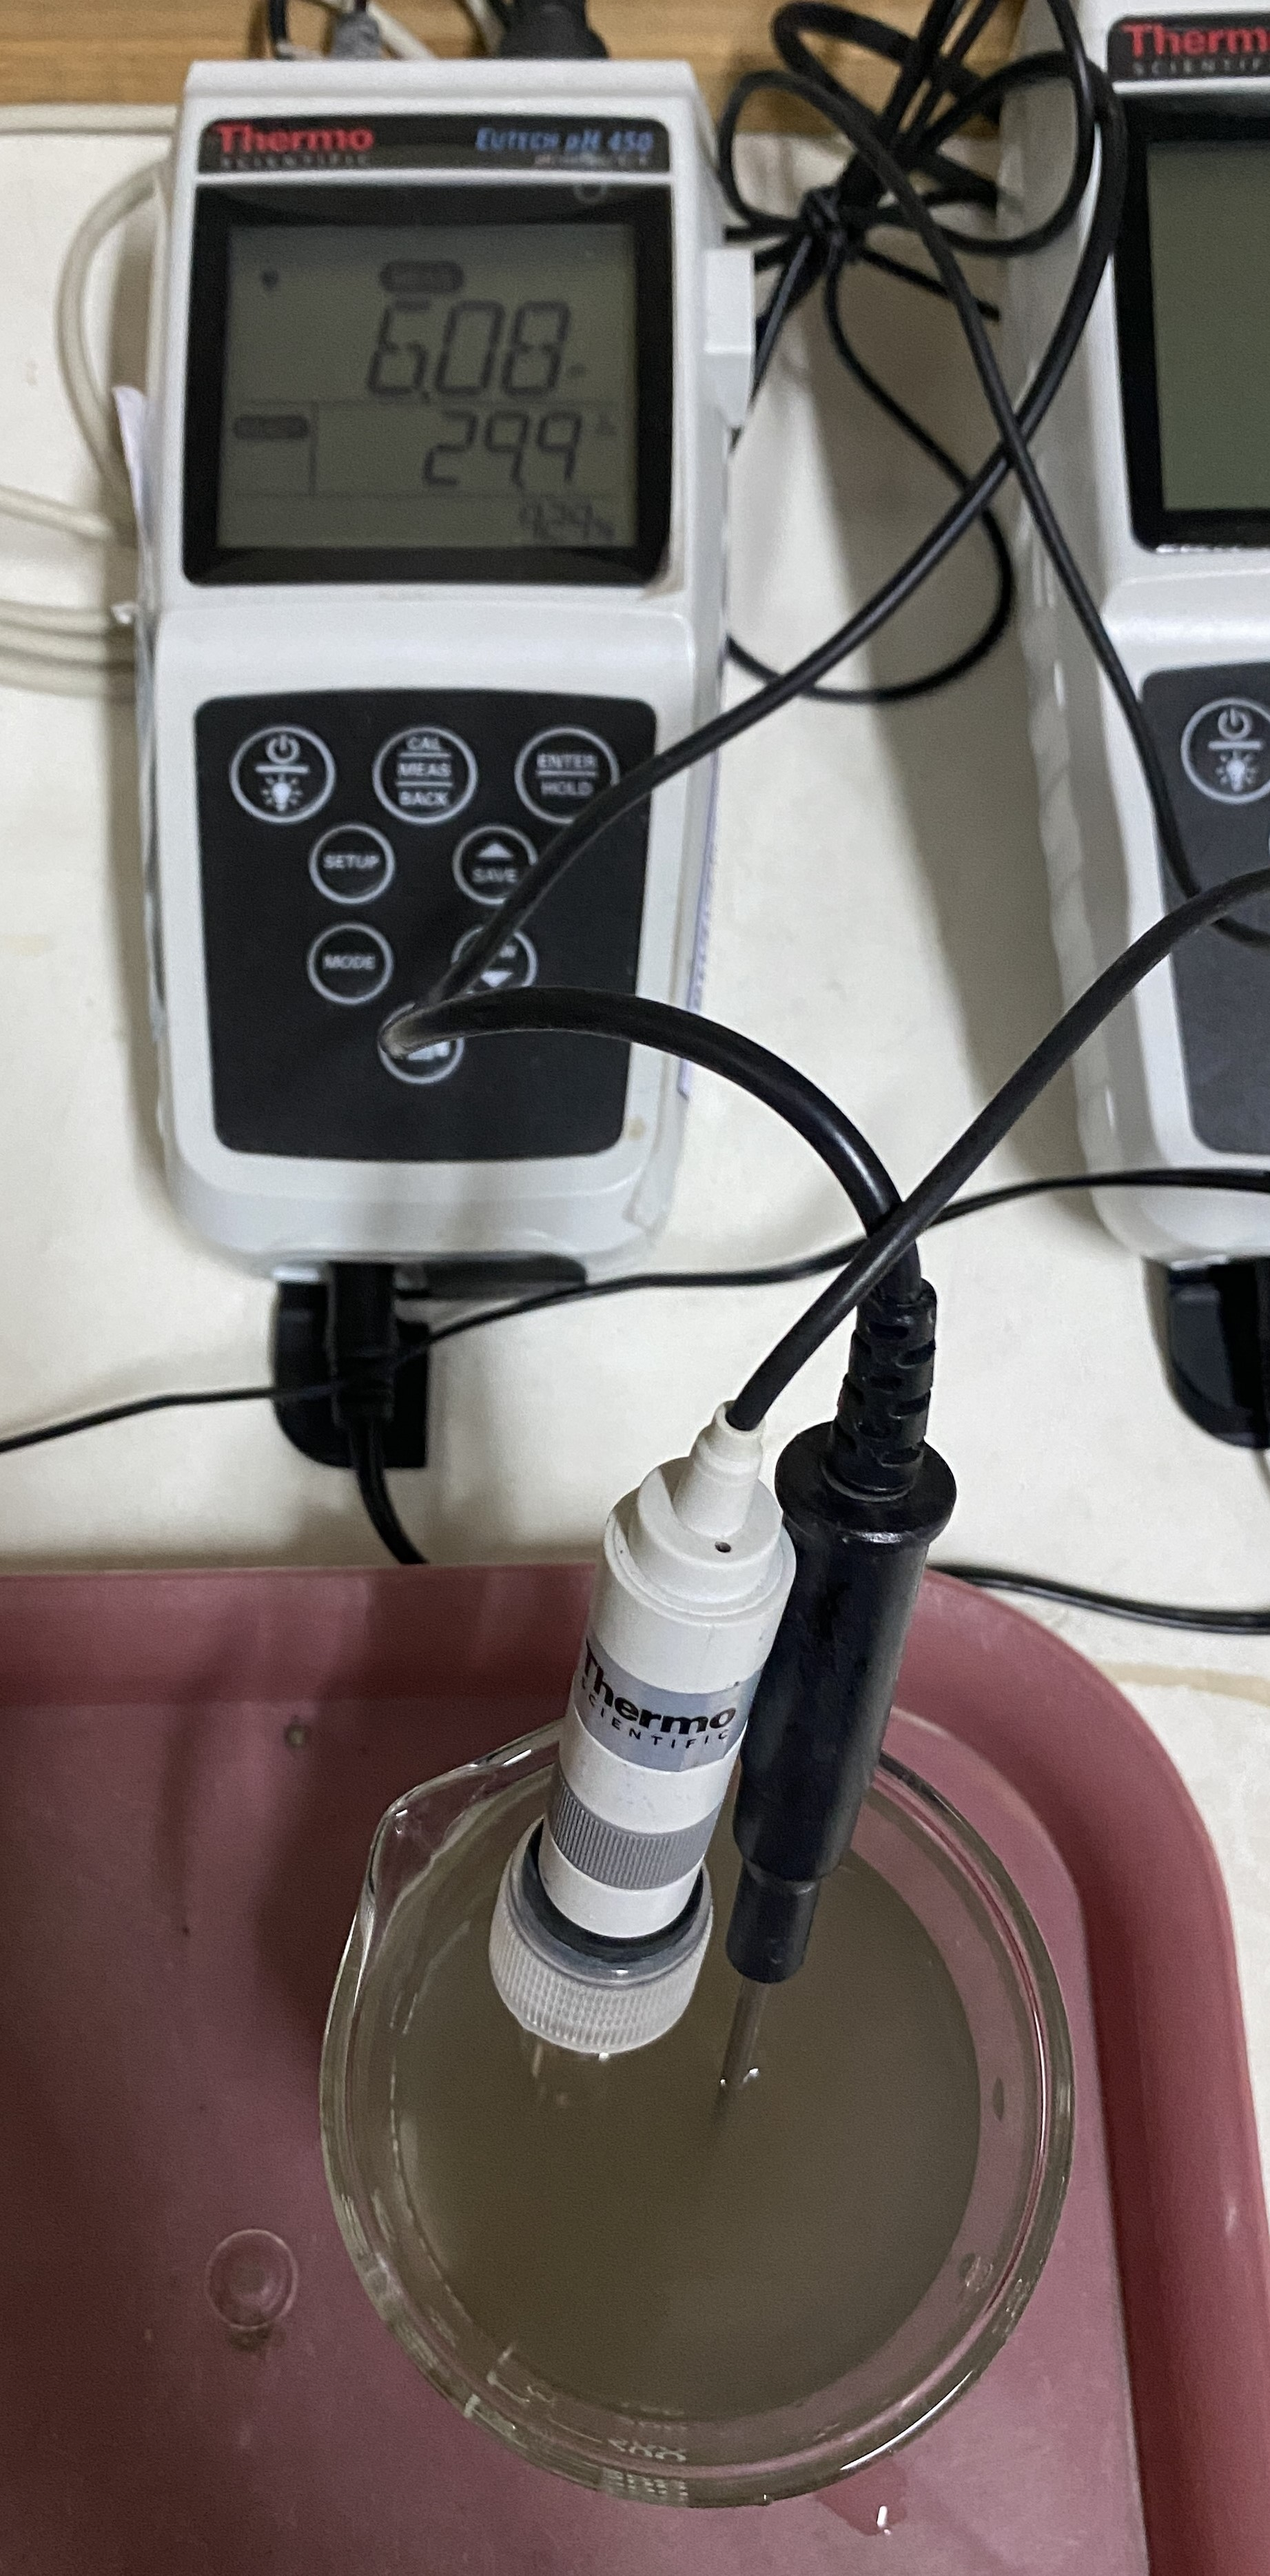
\includegraphics[width=.370\textwidth]{results/inlet_ph.JPG}\hfill
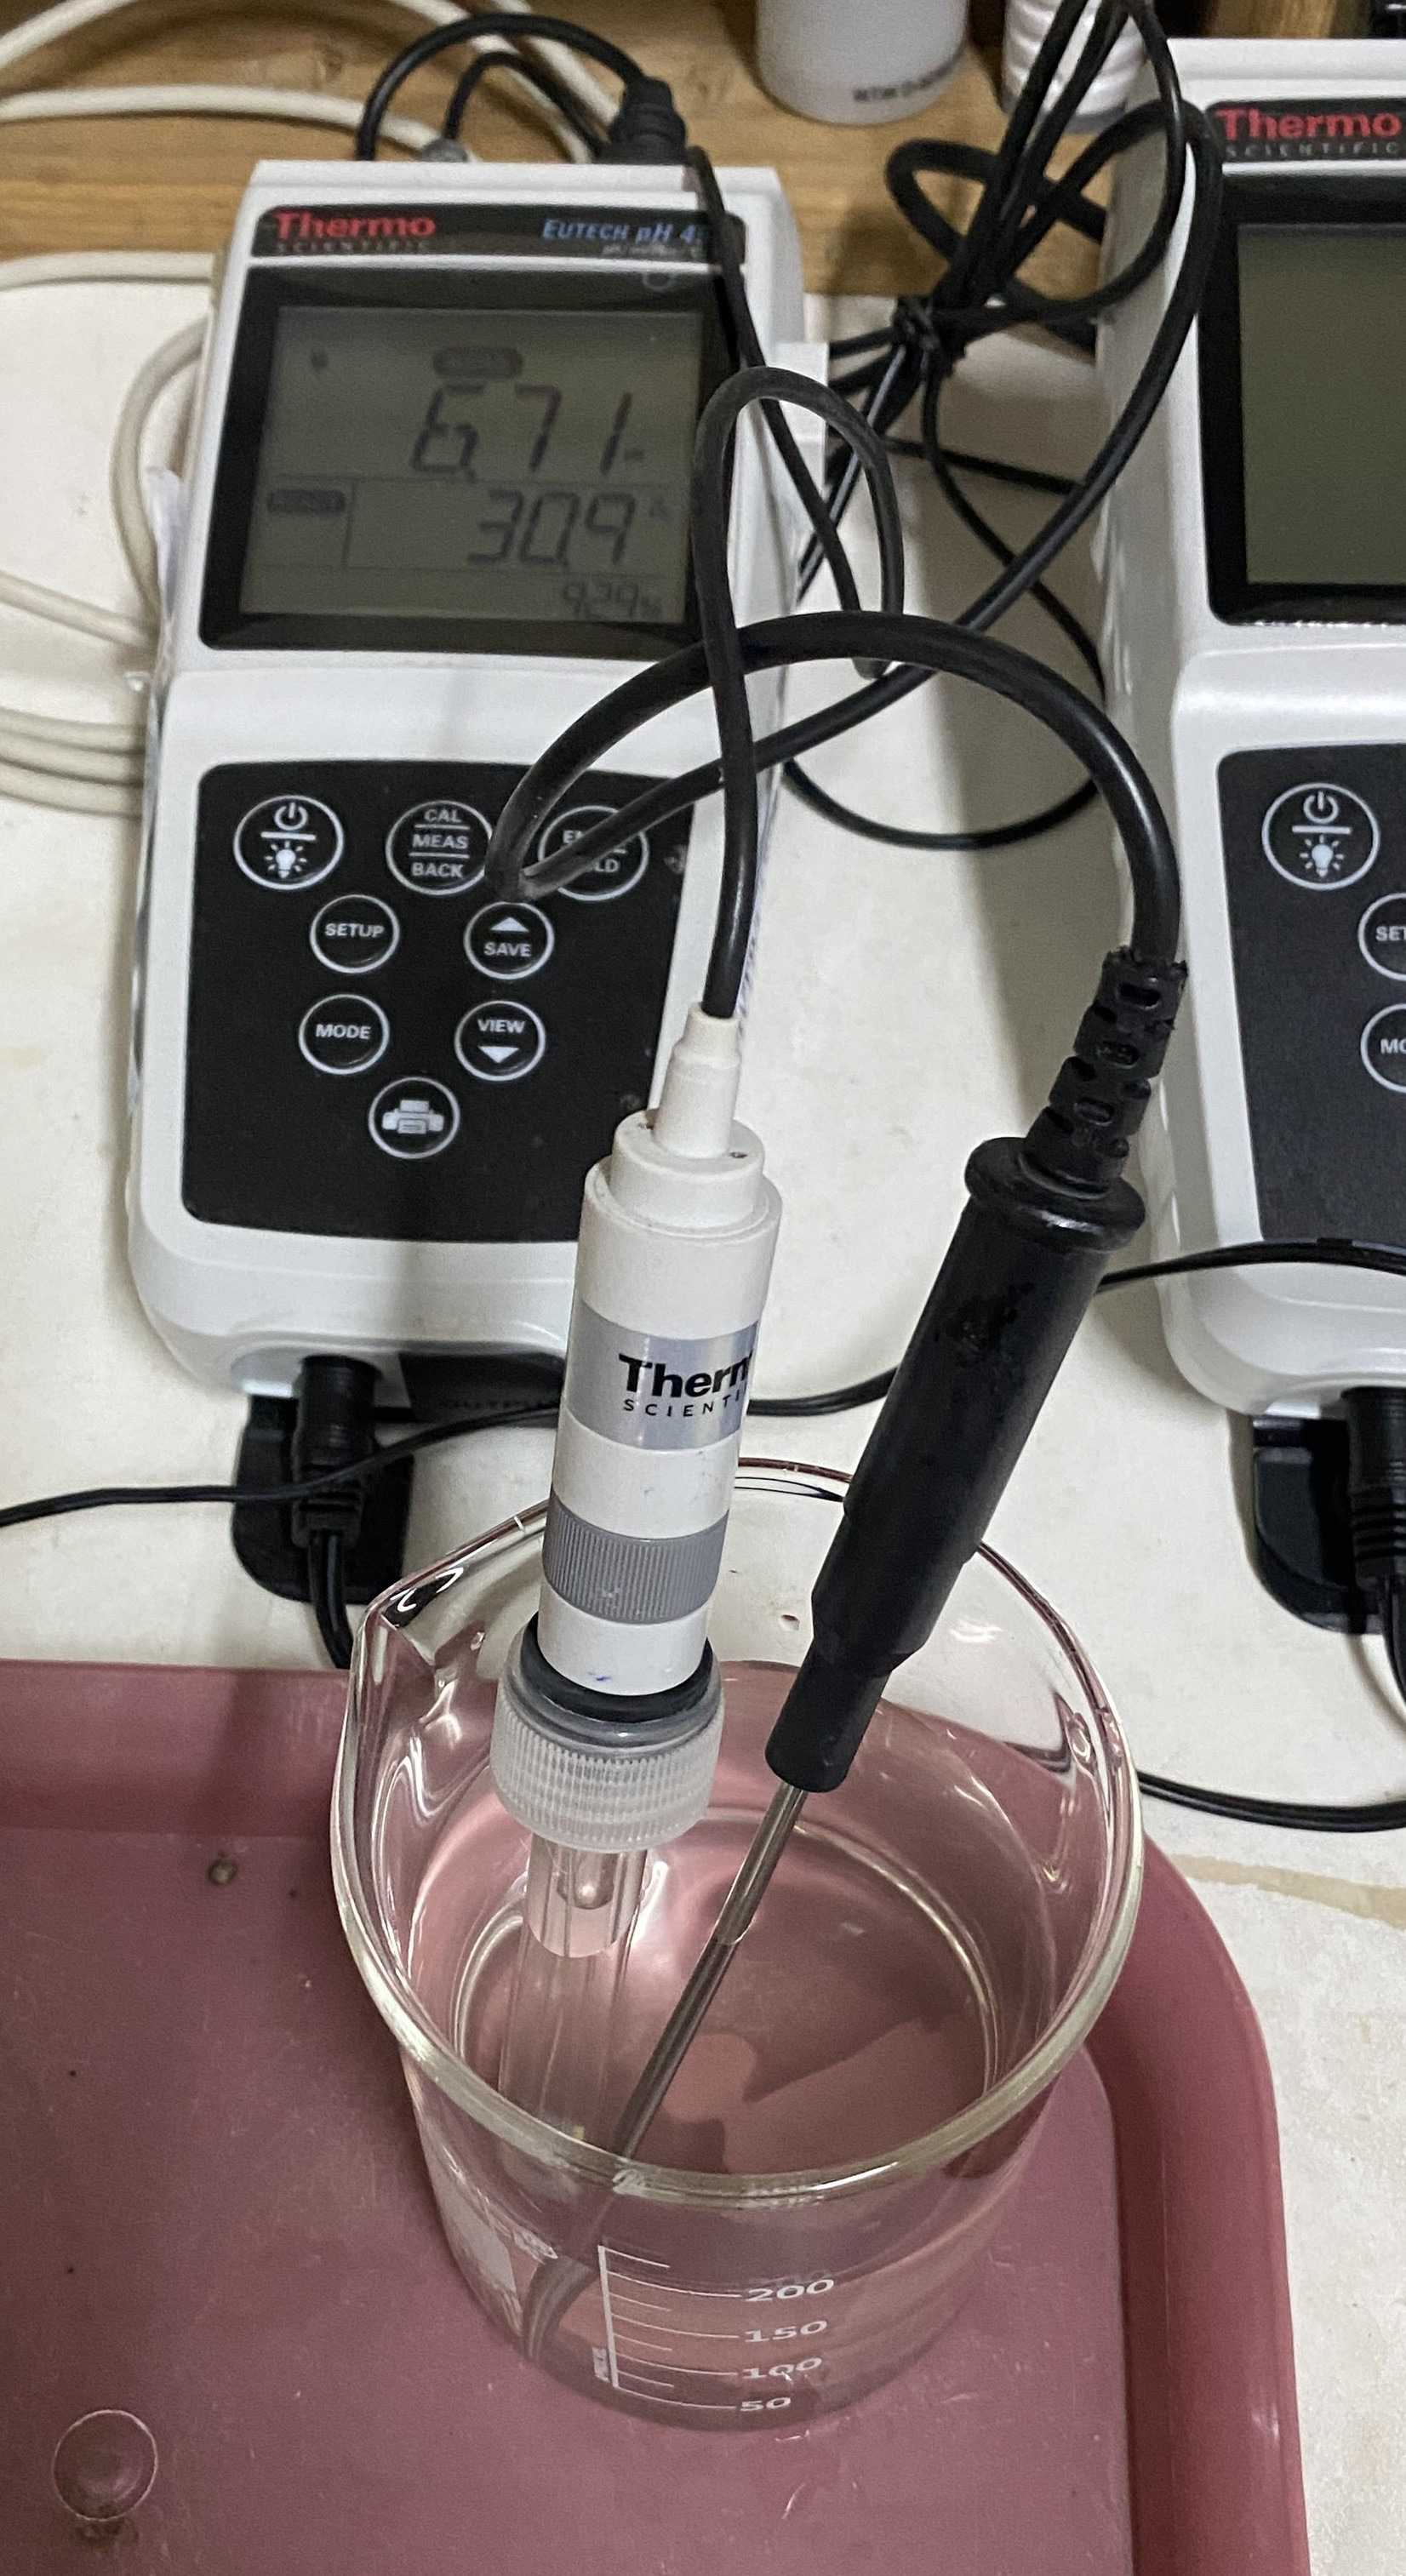
\includegraphics[width=.4\textwidth]{results/outlet_ph.JPG}\hfill

\caption{Measured pH and temperature of inlet and outlet}
\label{fig: pH and temperature}
\end{figure}


\begin{figure}[H]
\centering

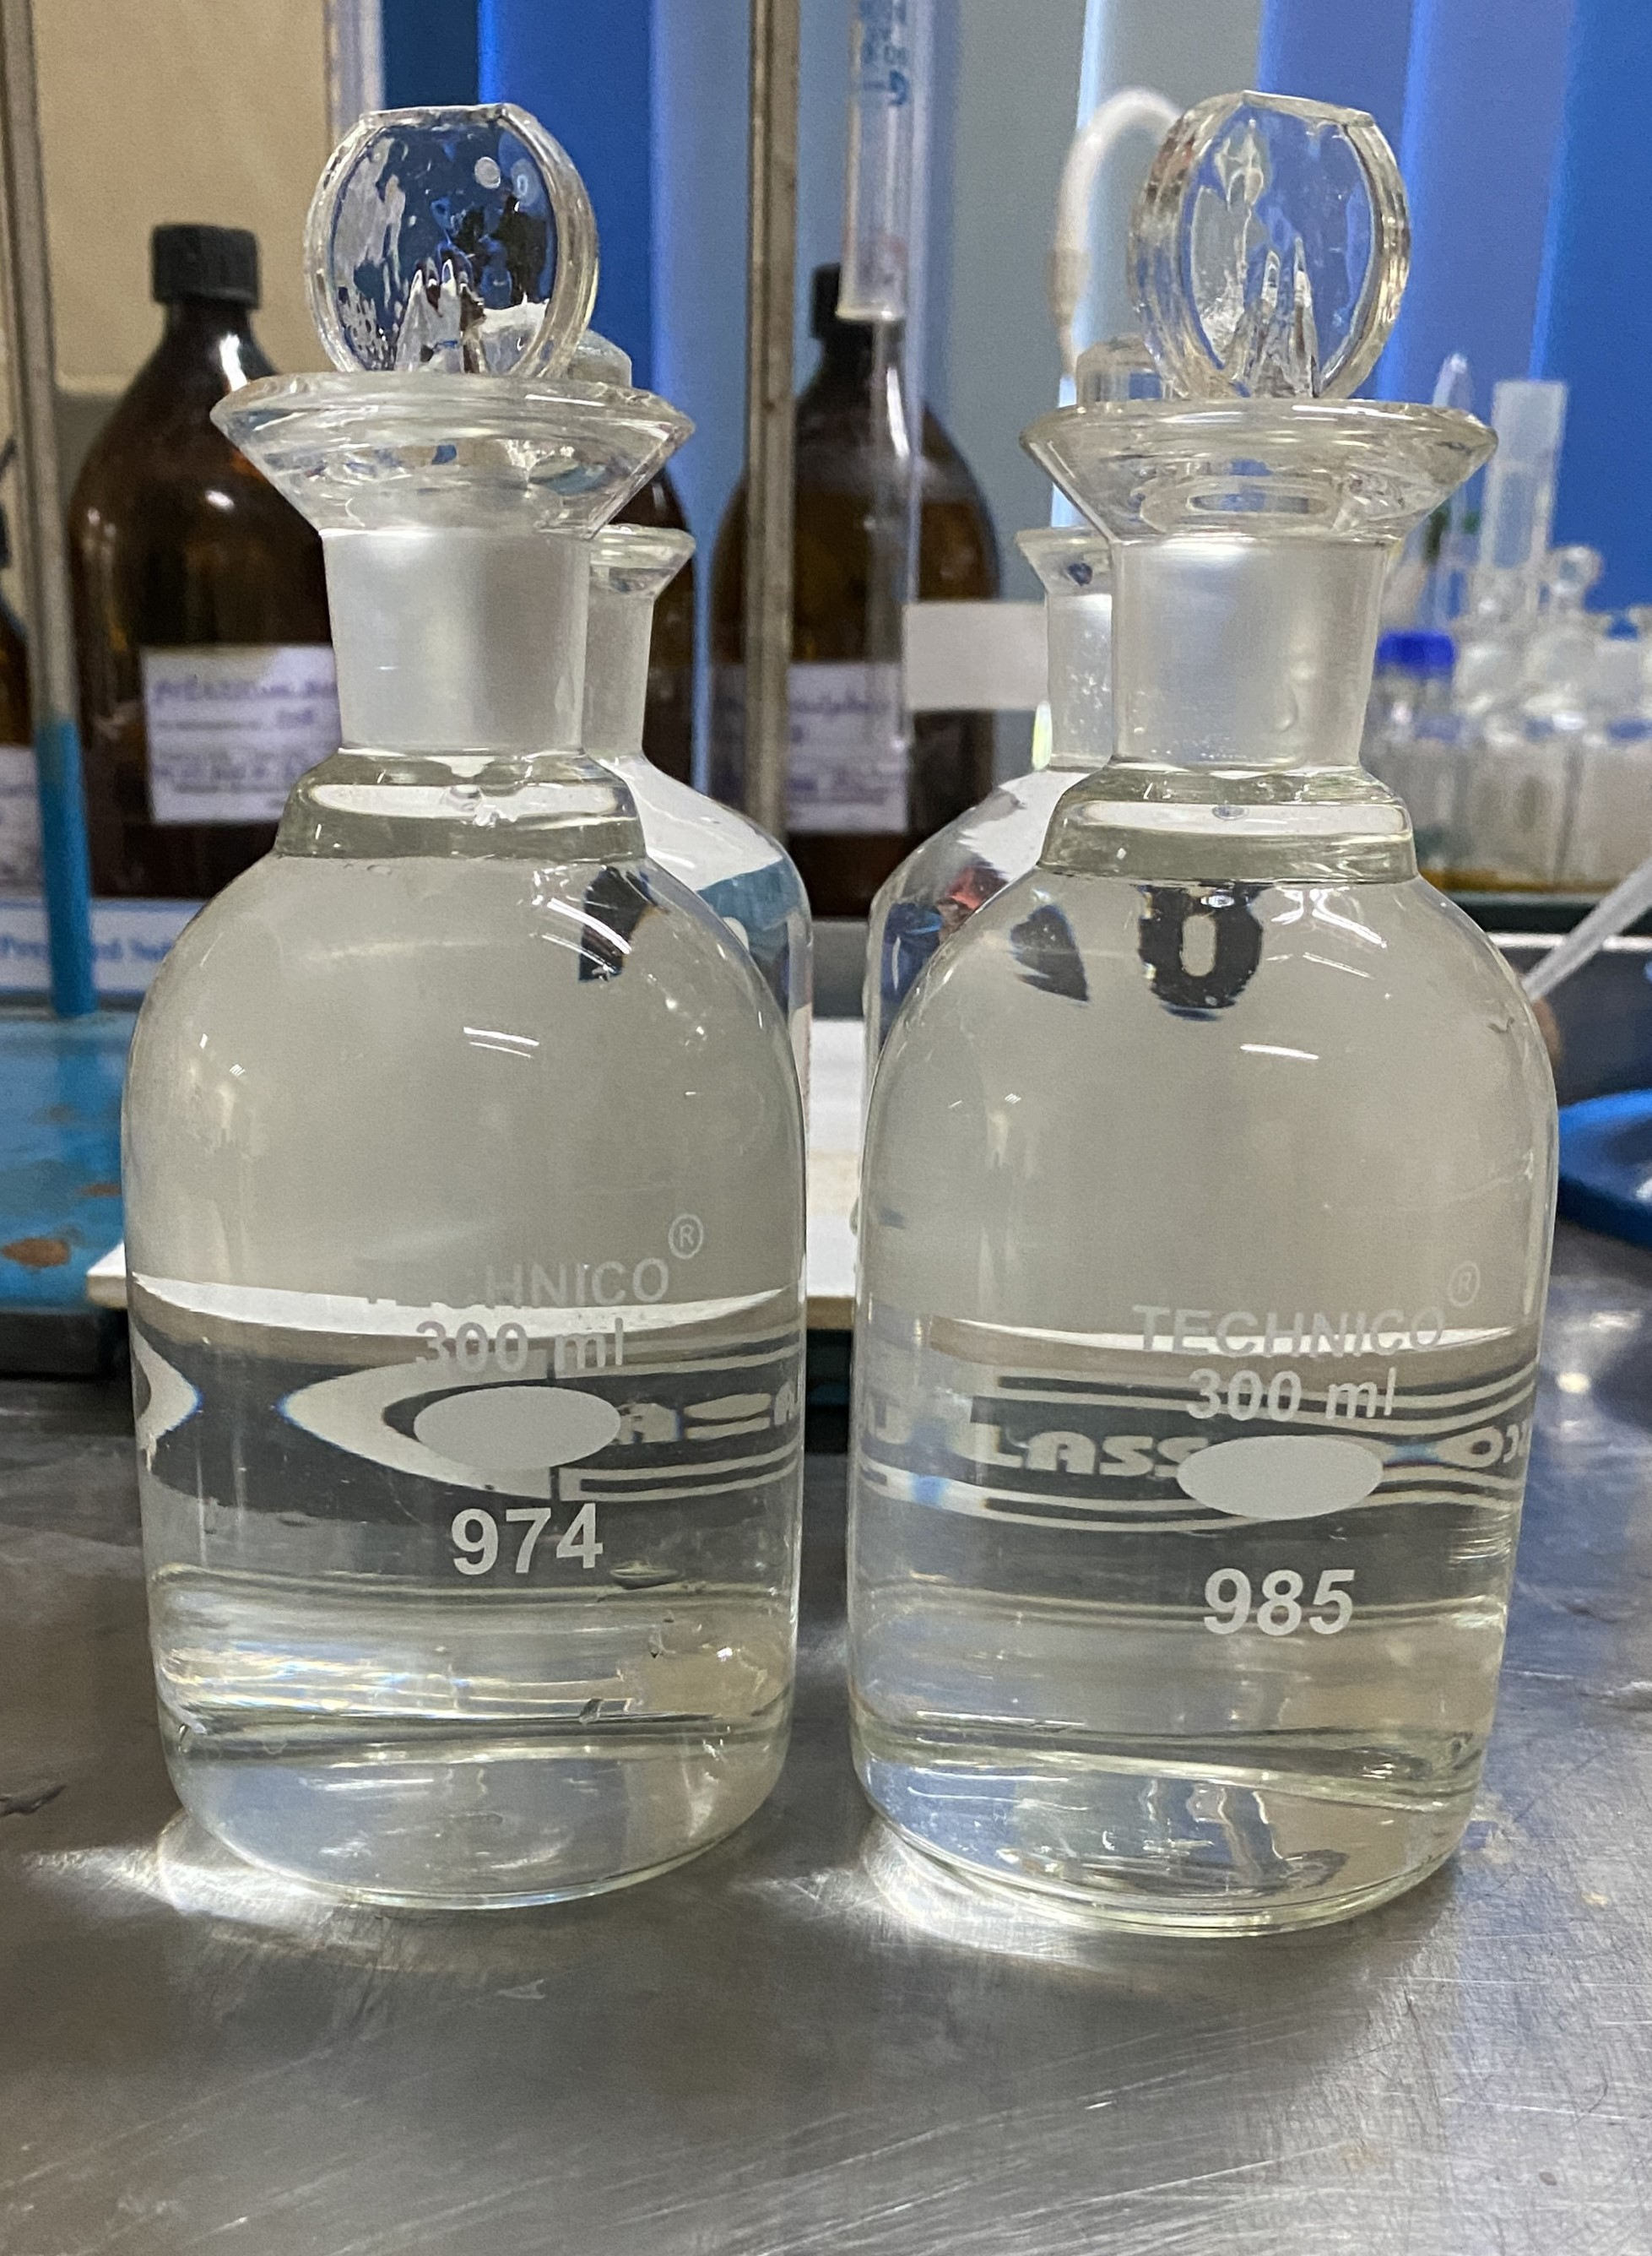
\includegraphics[width=.385\textwidth]{results/bod_before.JPG}\hfill
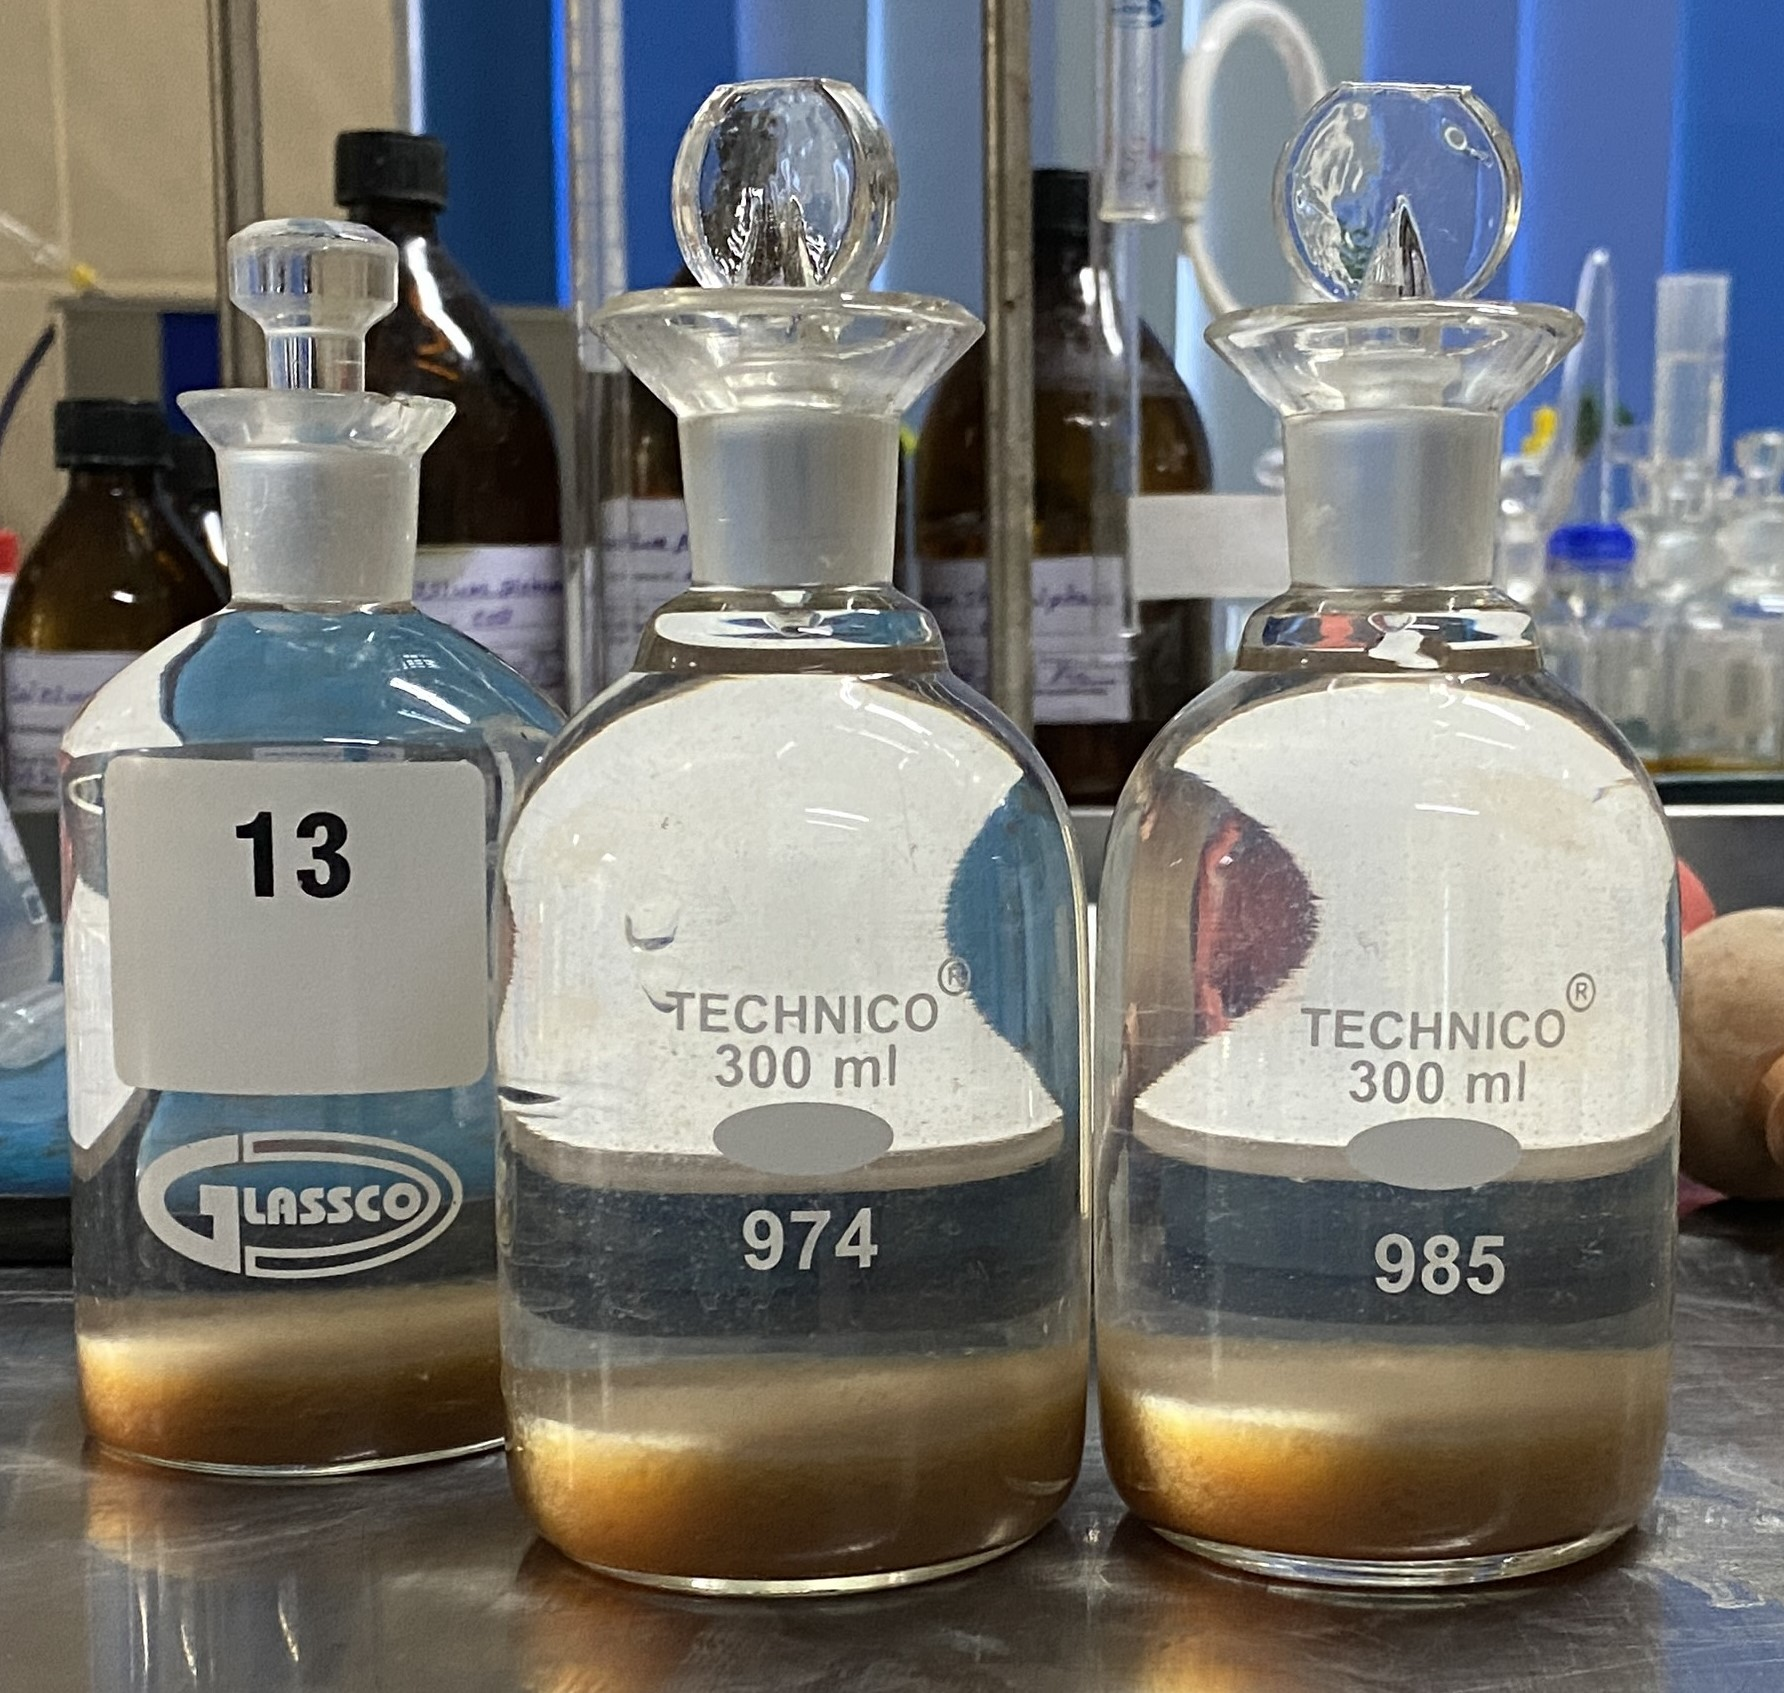
\includegraphics[width=.55\textwidth]{results/bod_precipitate.JPG}\hfill


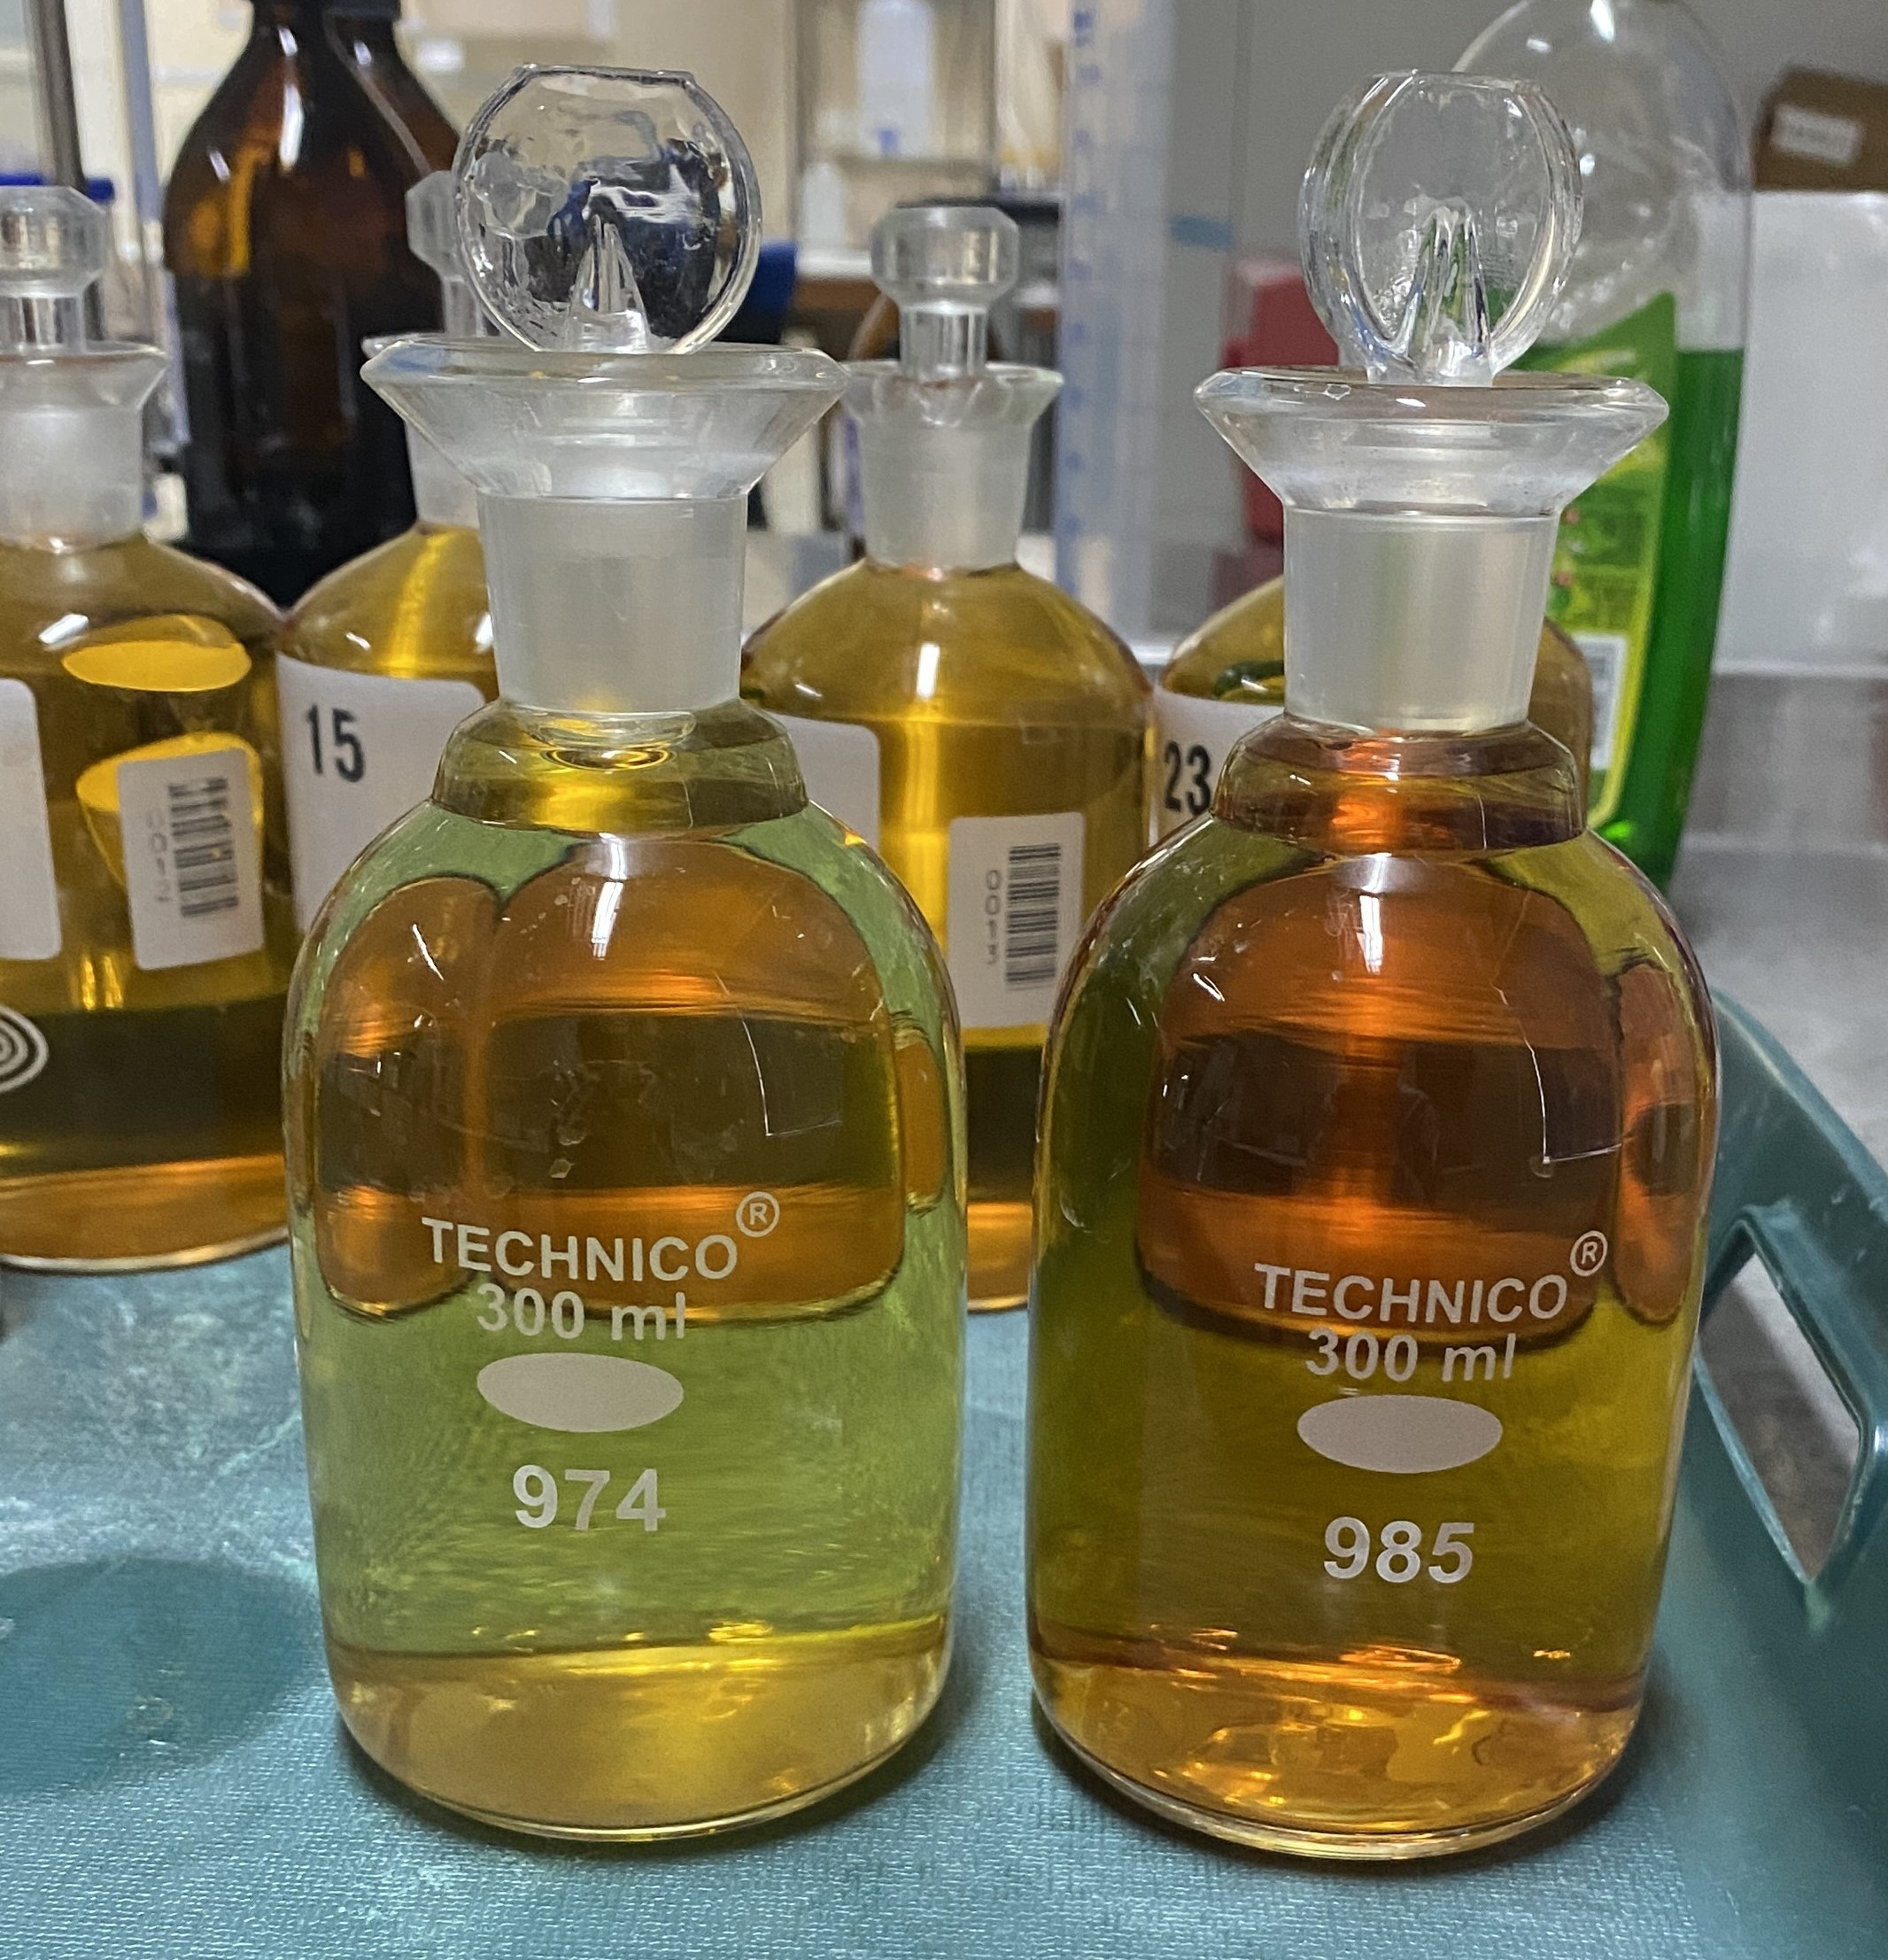
\includegraphics[width=.5\textwidth]{results/bod_after.JPG}\hfill


\caption{\ac{BOD5} analysed samples of inlet and outlet during 5 days}
\label{fig: bod_before_after_samples}
\end{figure}

\begin{figure}[H]
\centering

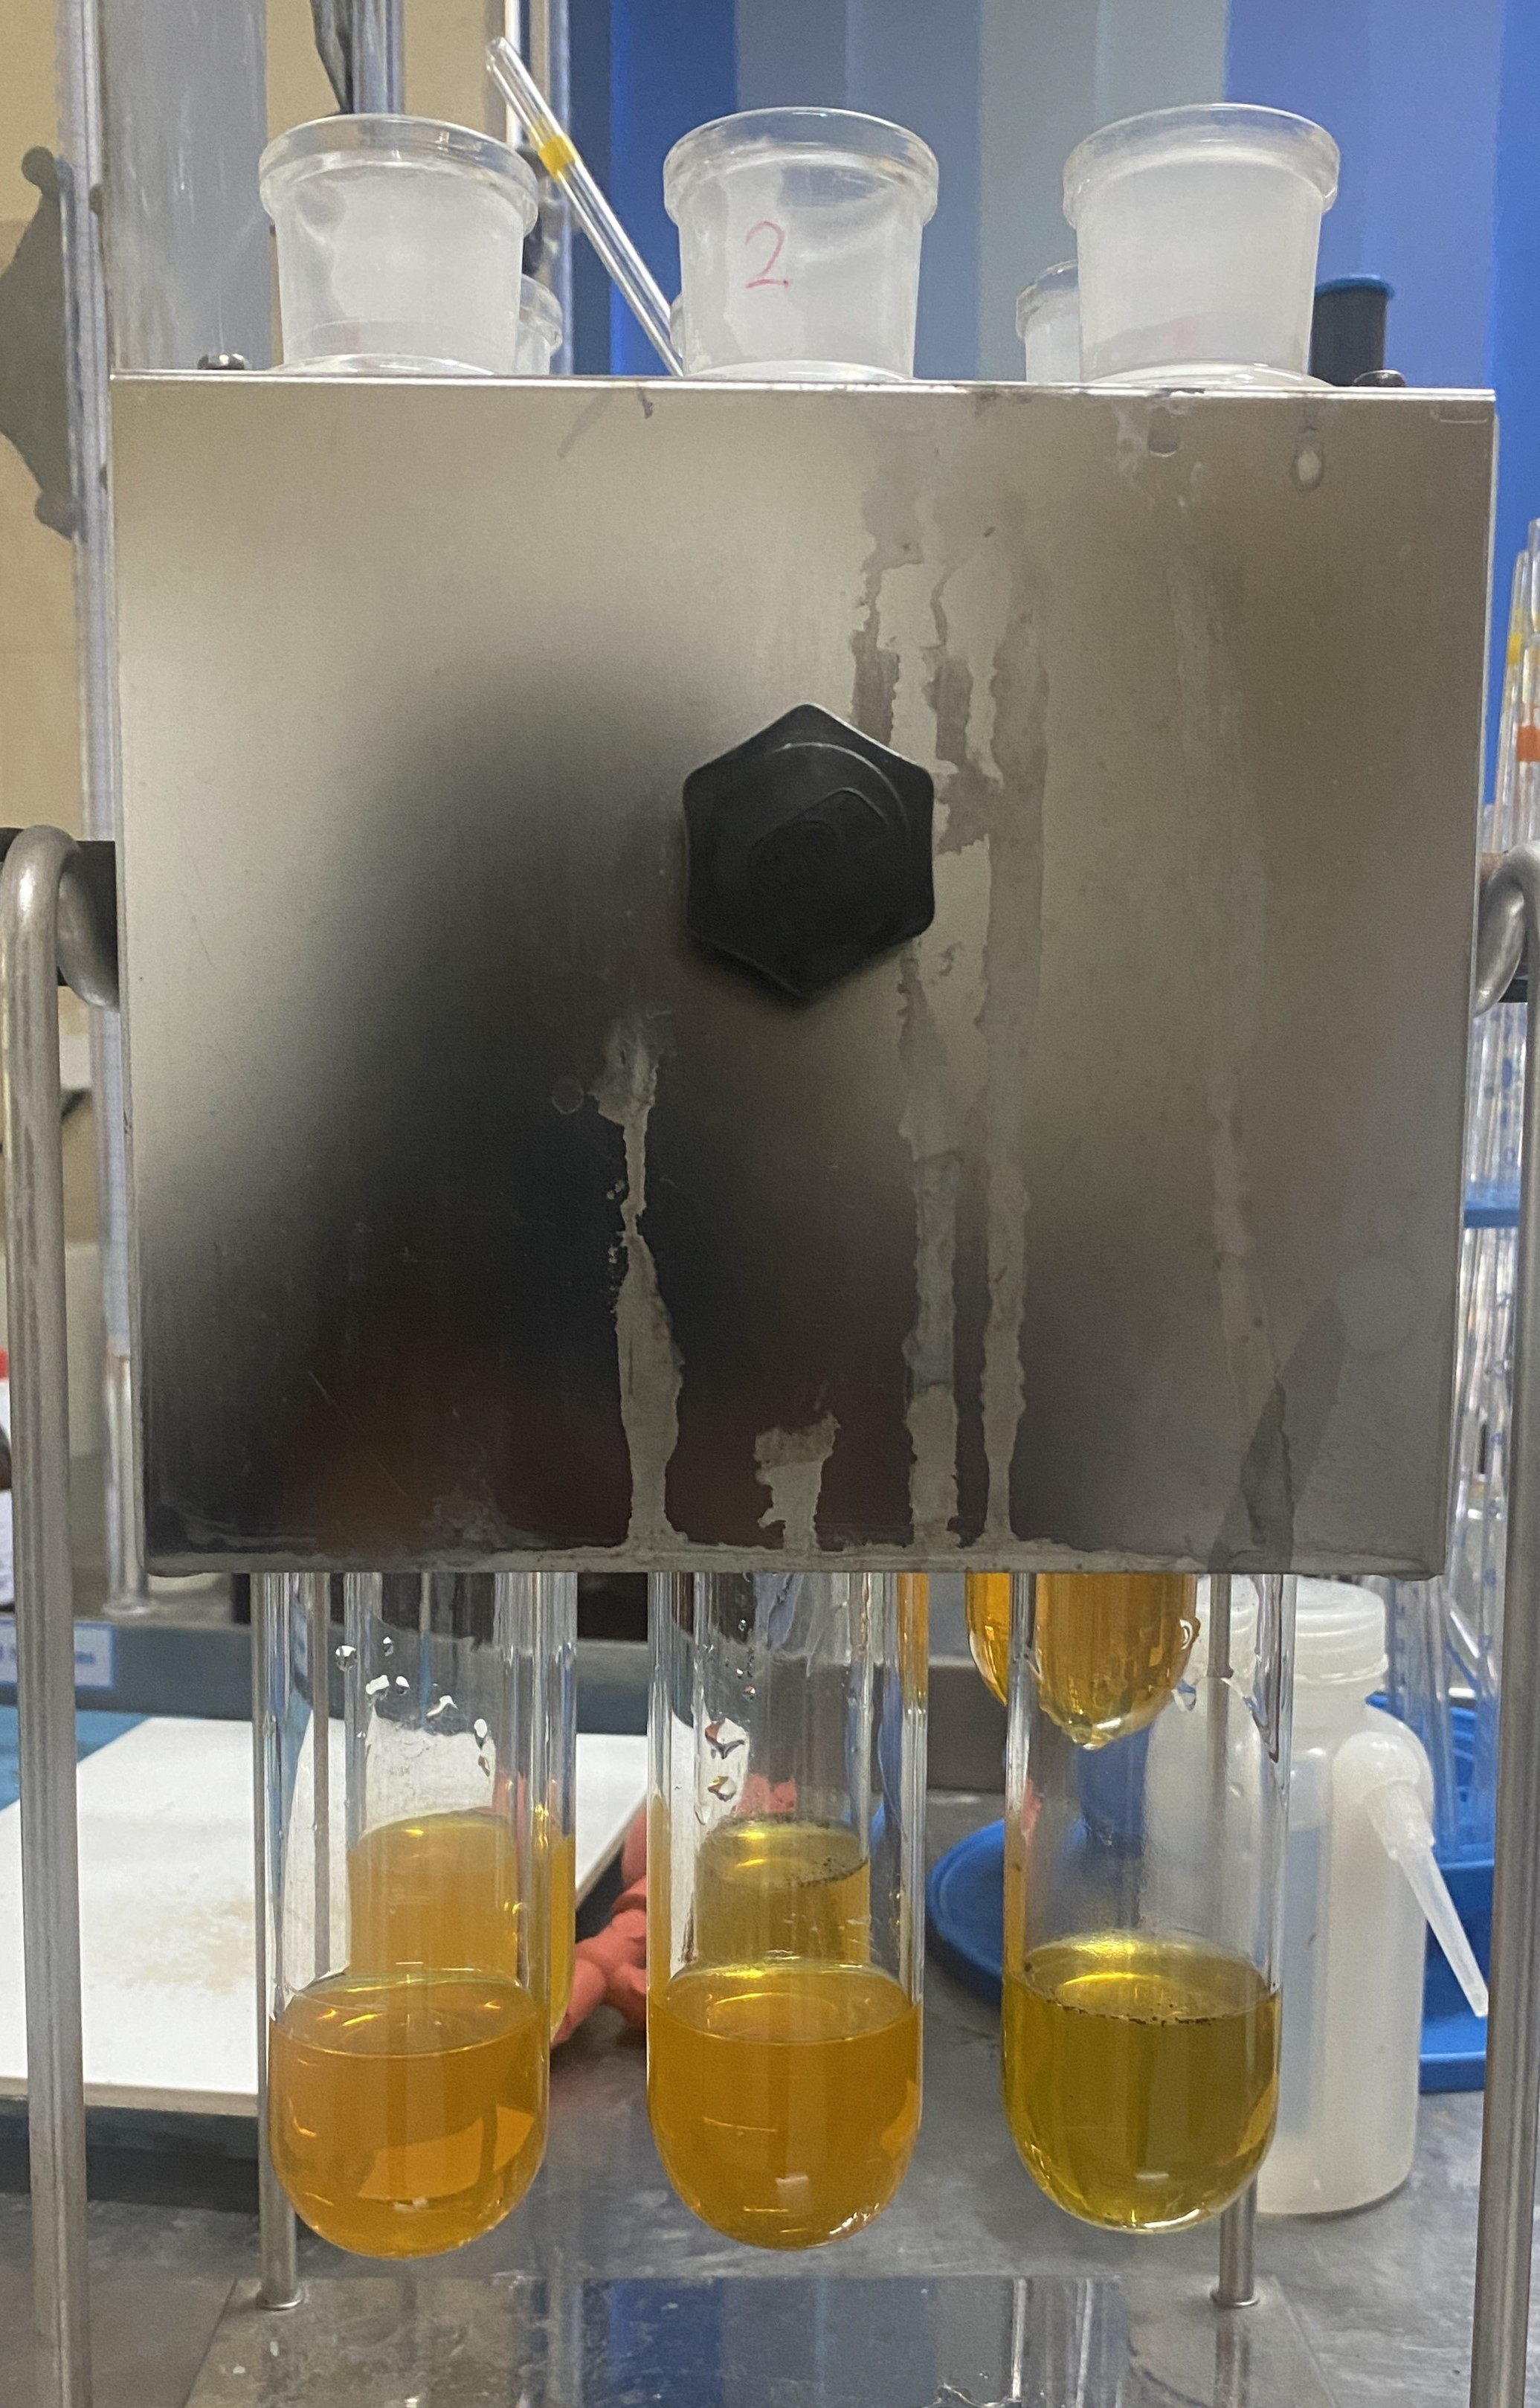
\includegraphics[width=.3\textwidth]{results/cod_samples.JPG}\hfill
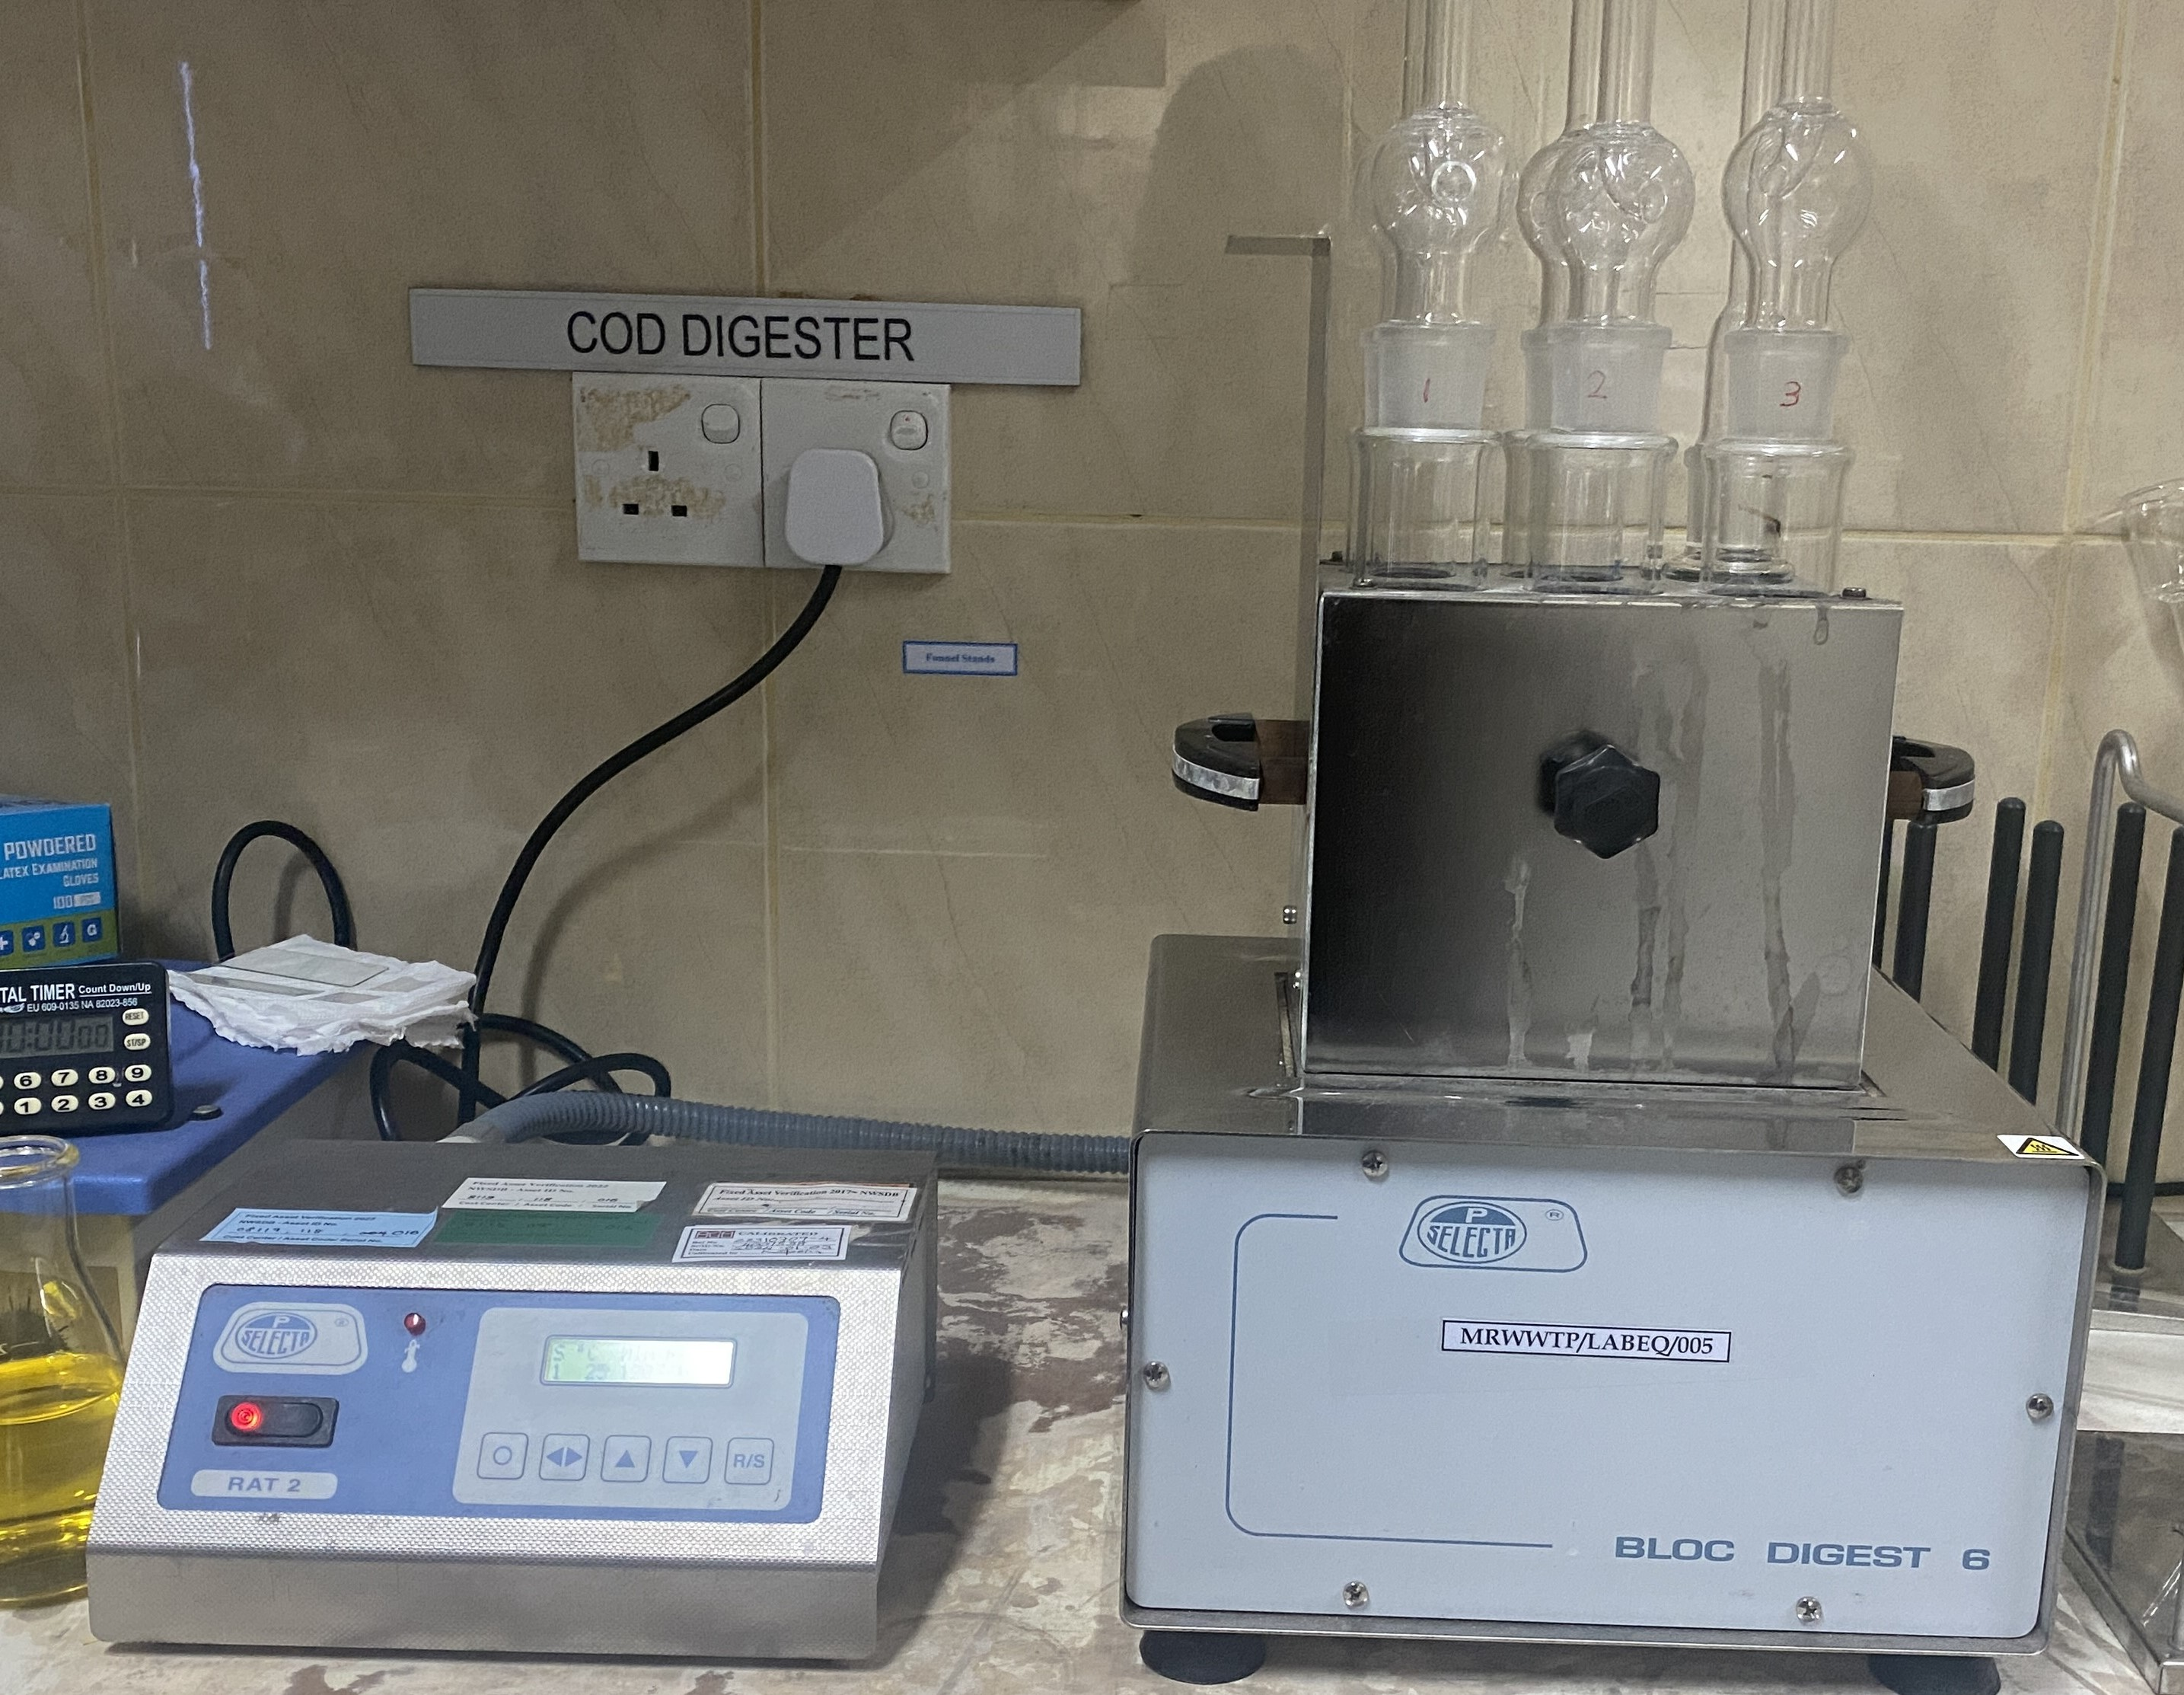
\includegraphics[width=.6\textwidth]{results/cod_digester.JPG}\hfill

\caption{\ac{COD} analyzed samples of the inlet and outlet}
\label{fig: cod_analyzed_sample}
\end{figure}

\begin{figure}[H]
\centering
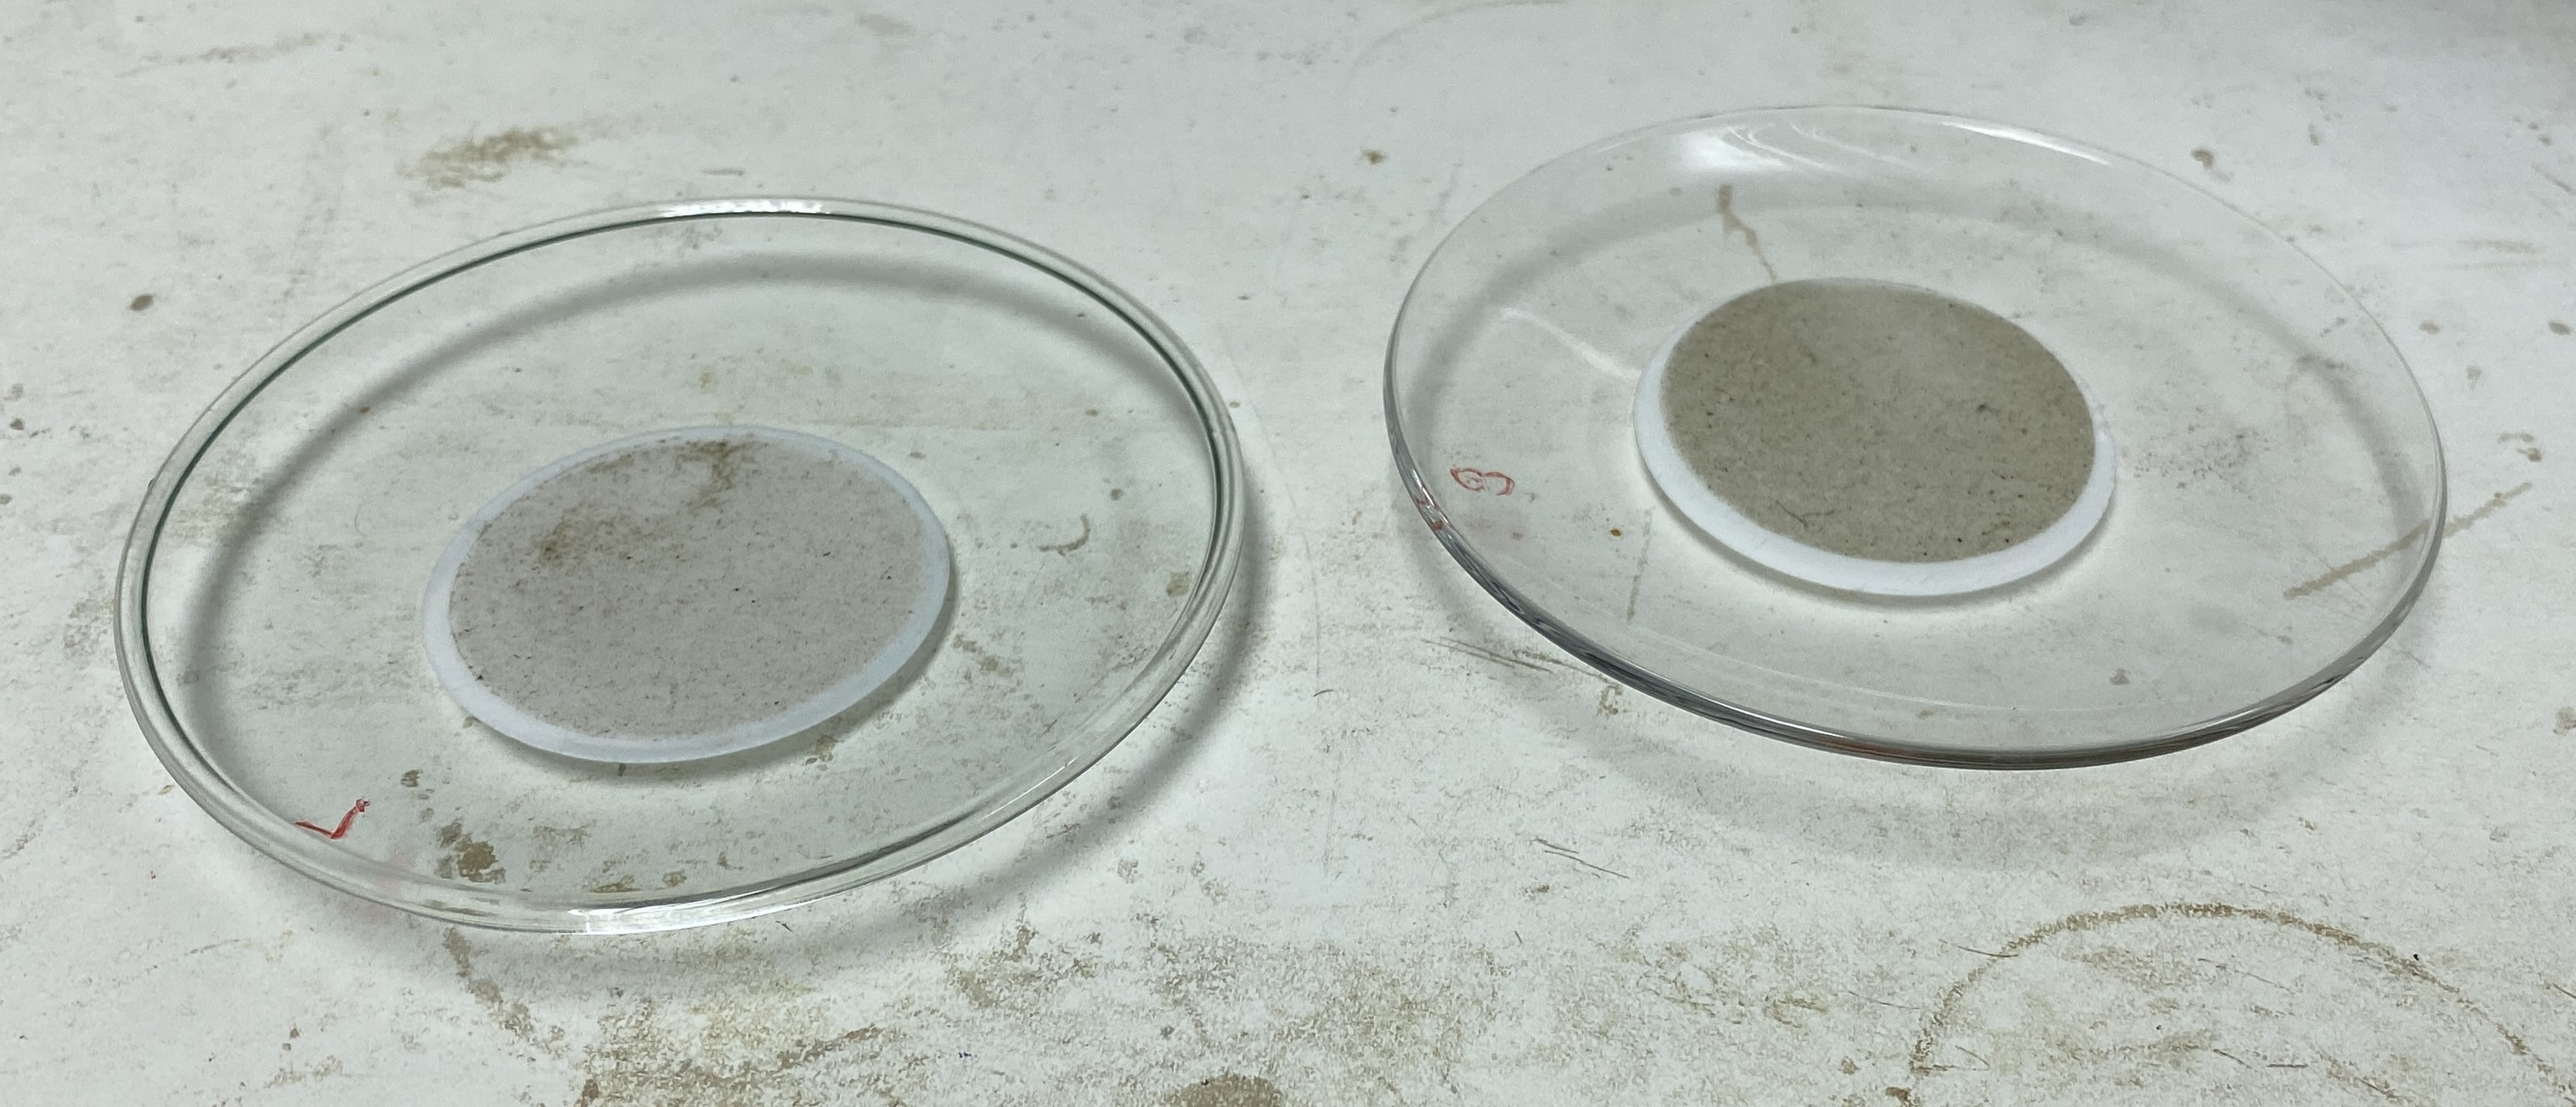
\includegraphics[width=0.77\linewidth]{results/tss_analyze_sample.JPG}
\caption{Filtered samples to analyze the \ac{TSS} of the outlet and inlet}
\label{fig:tss_analyze_sample}
\end{figure}


\begin{figure}[H]
\centering
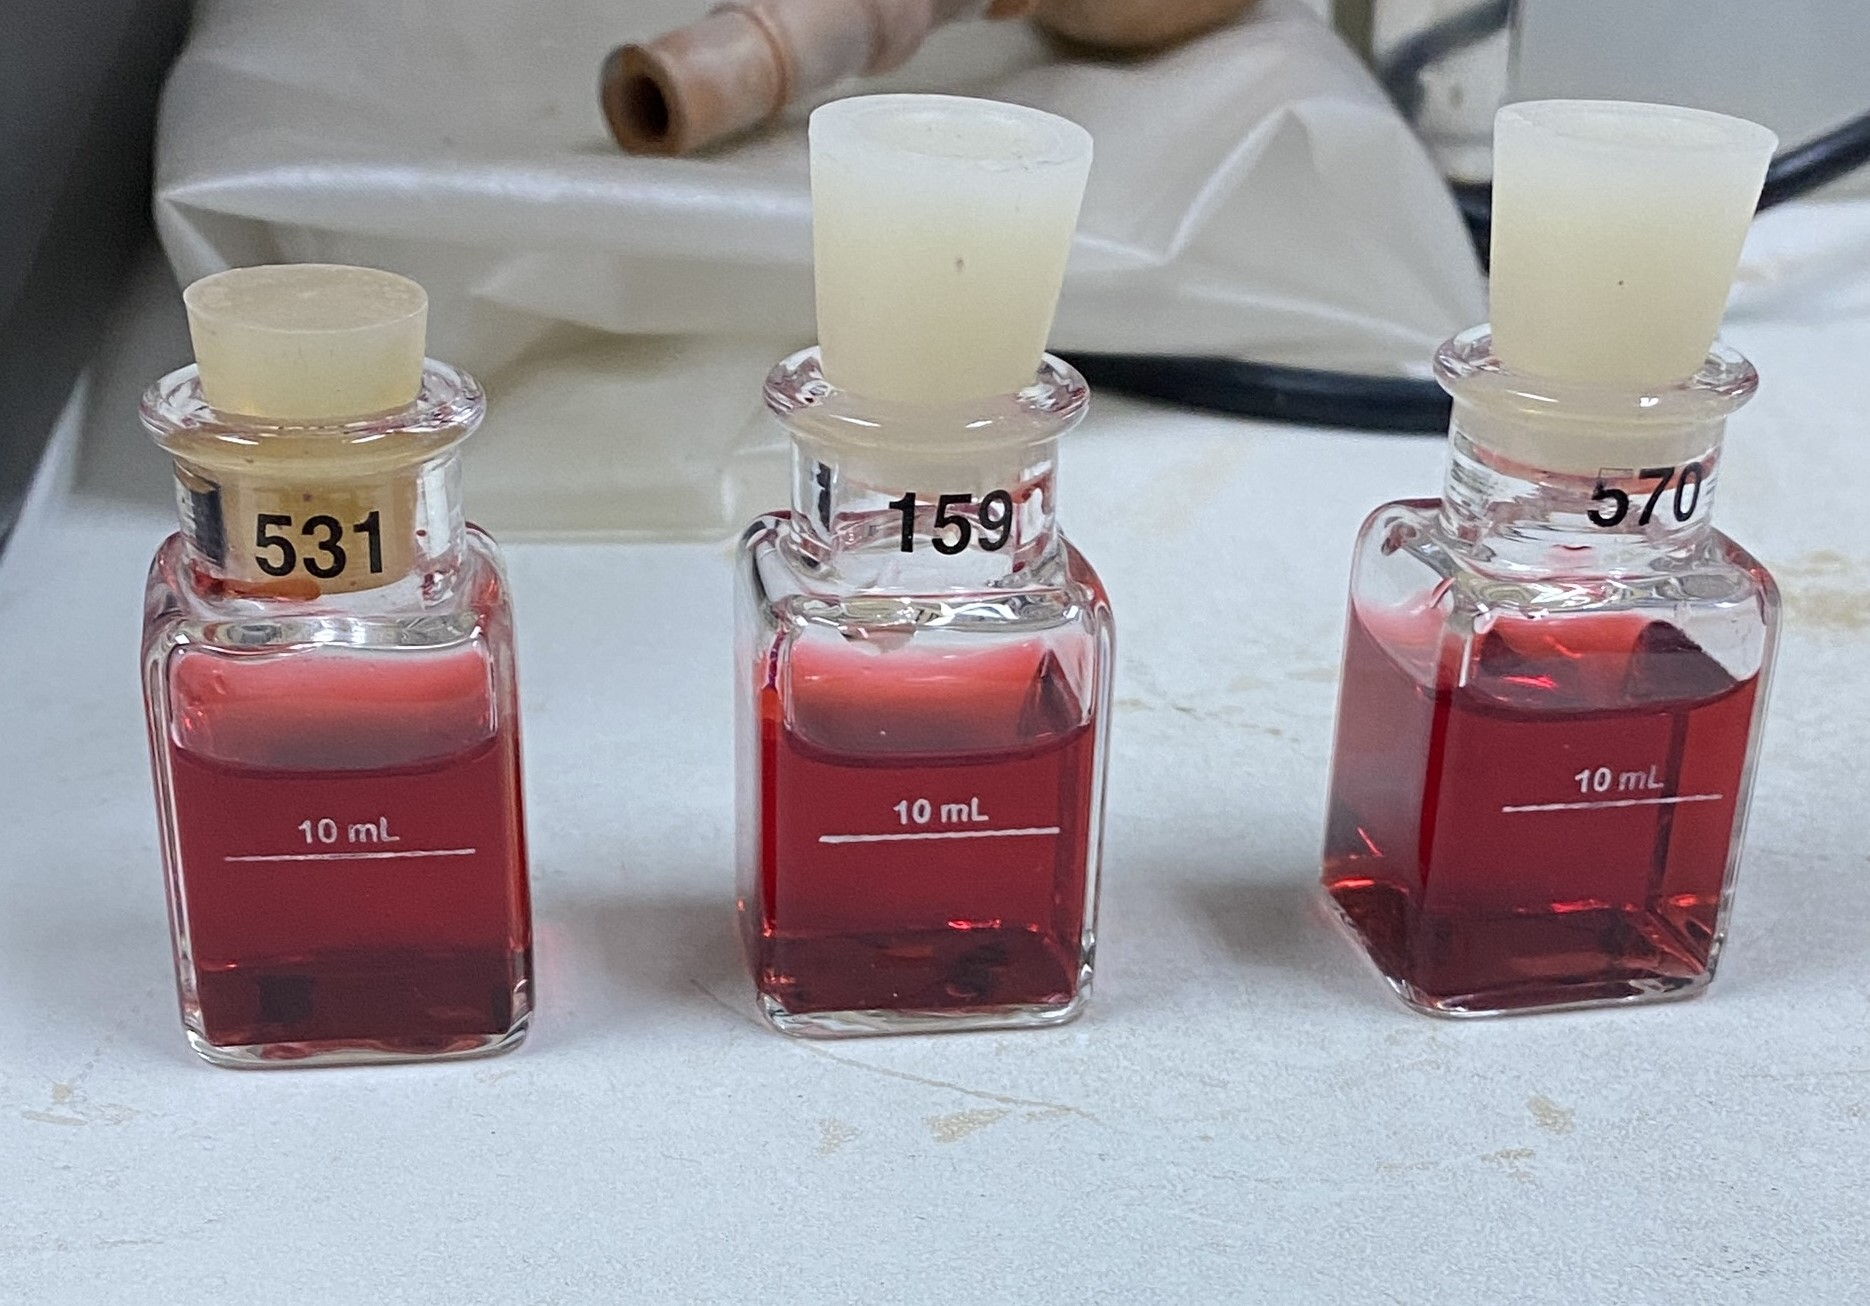
\includegraphics[width=0.6\linewidth]{results/fluoride_analyze_sample.JPG}
\caption{Samples prepared to analyze fluoride in the inlet and outlet}
\label{fig:fluoride_analyze_sample}
\end{figure}

\begin{figure}[H]
\centering

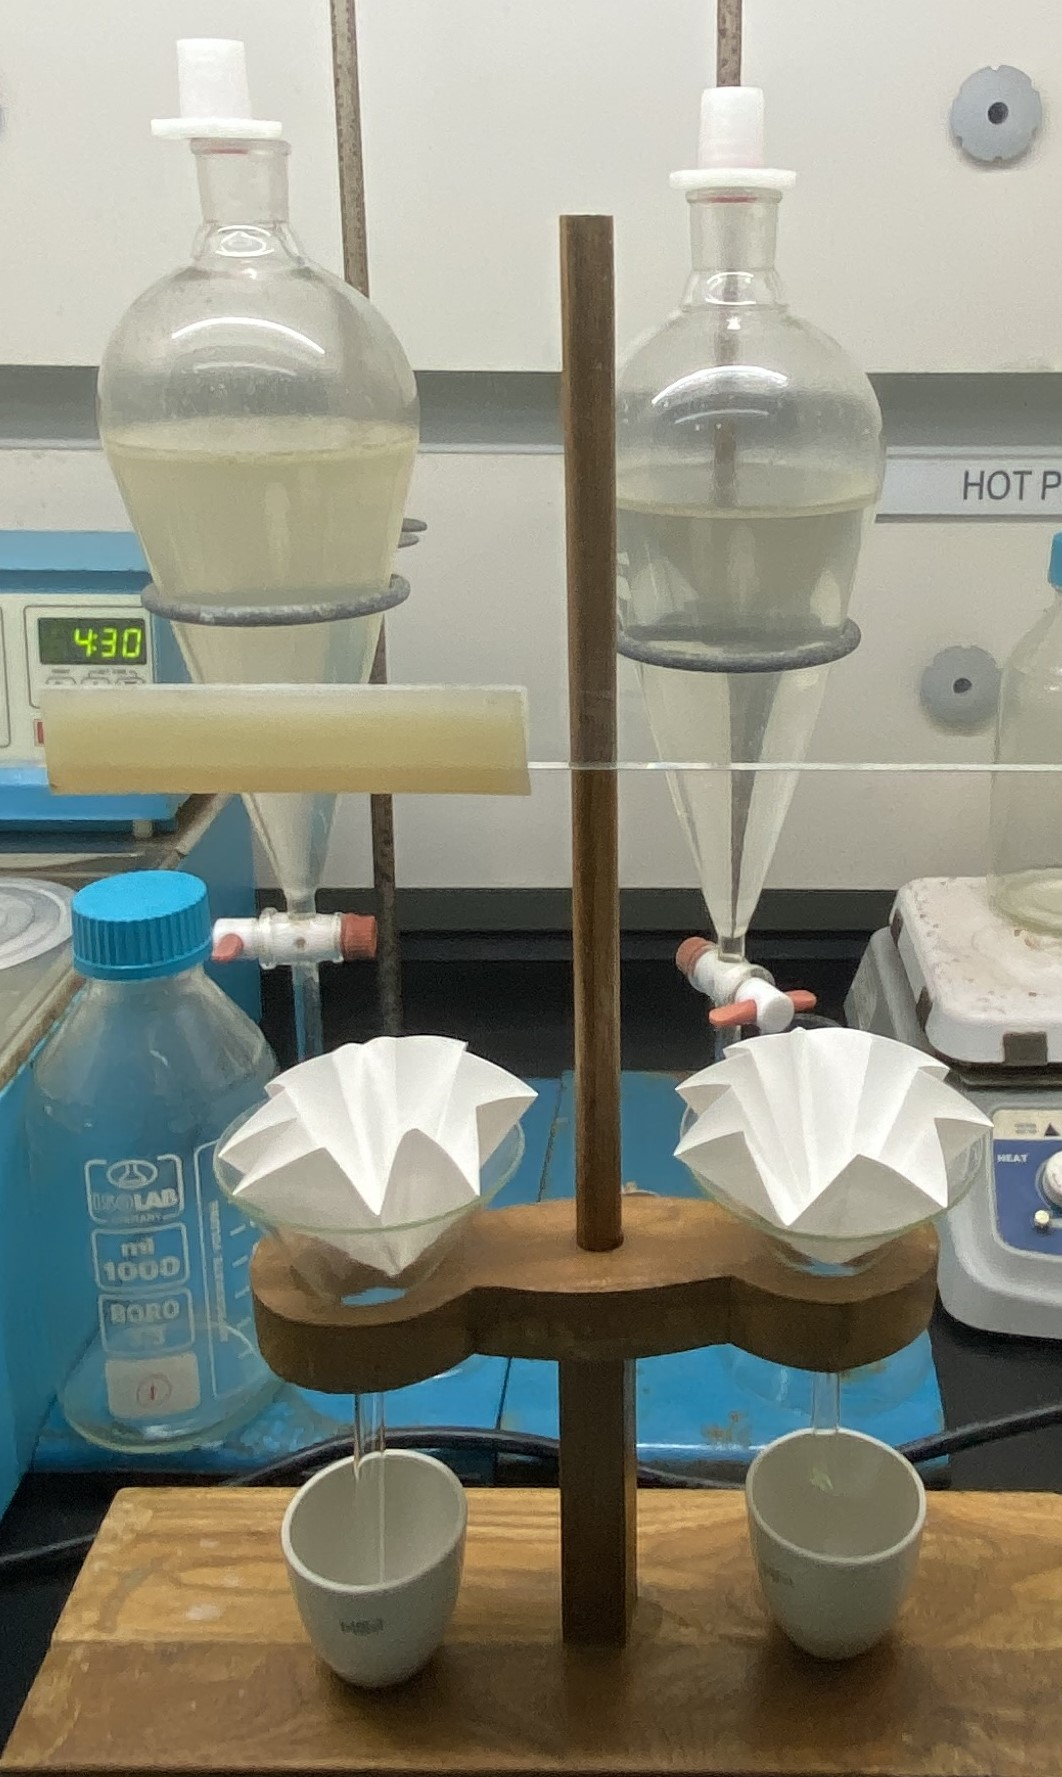
\includegraphics[width=.36\textwidth]{results/oil _and_grease_analyze_sample.JPG}\hfill
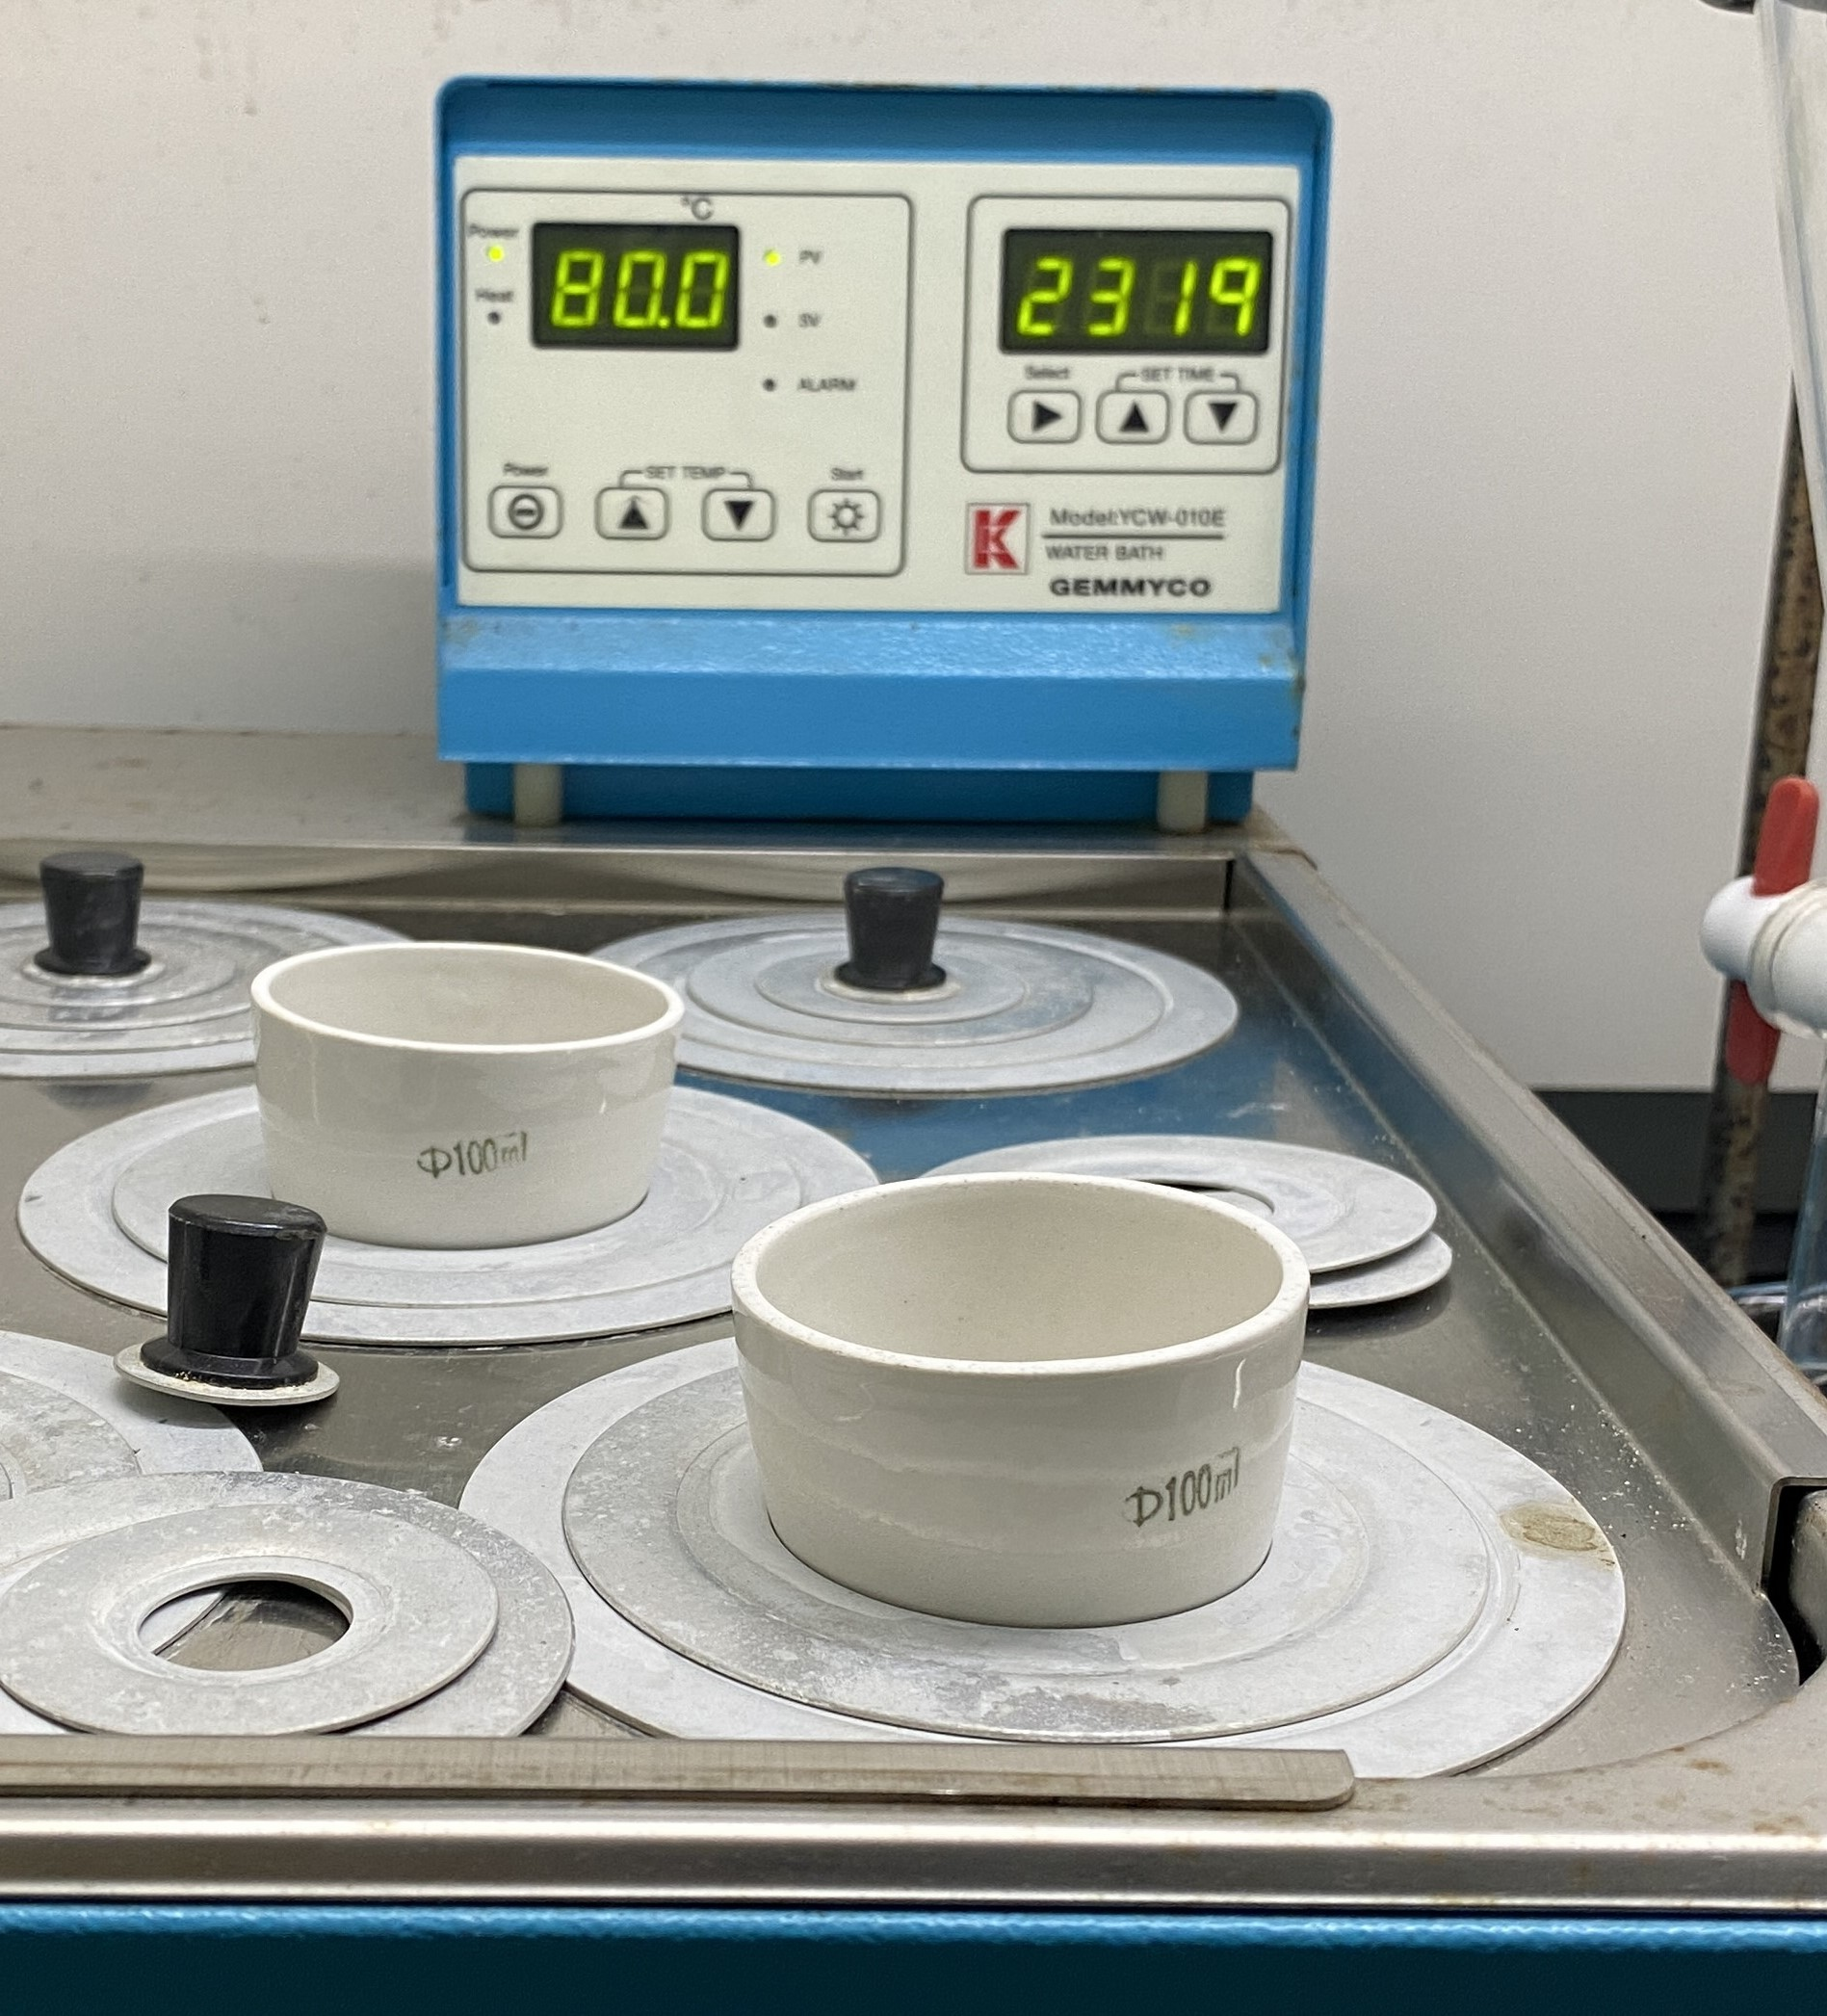
\includegraphics[width=.55\textwidth]{results/waterbath_oil_and_grease_sample.JPG}\hfill

\vspace{3mm}

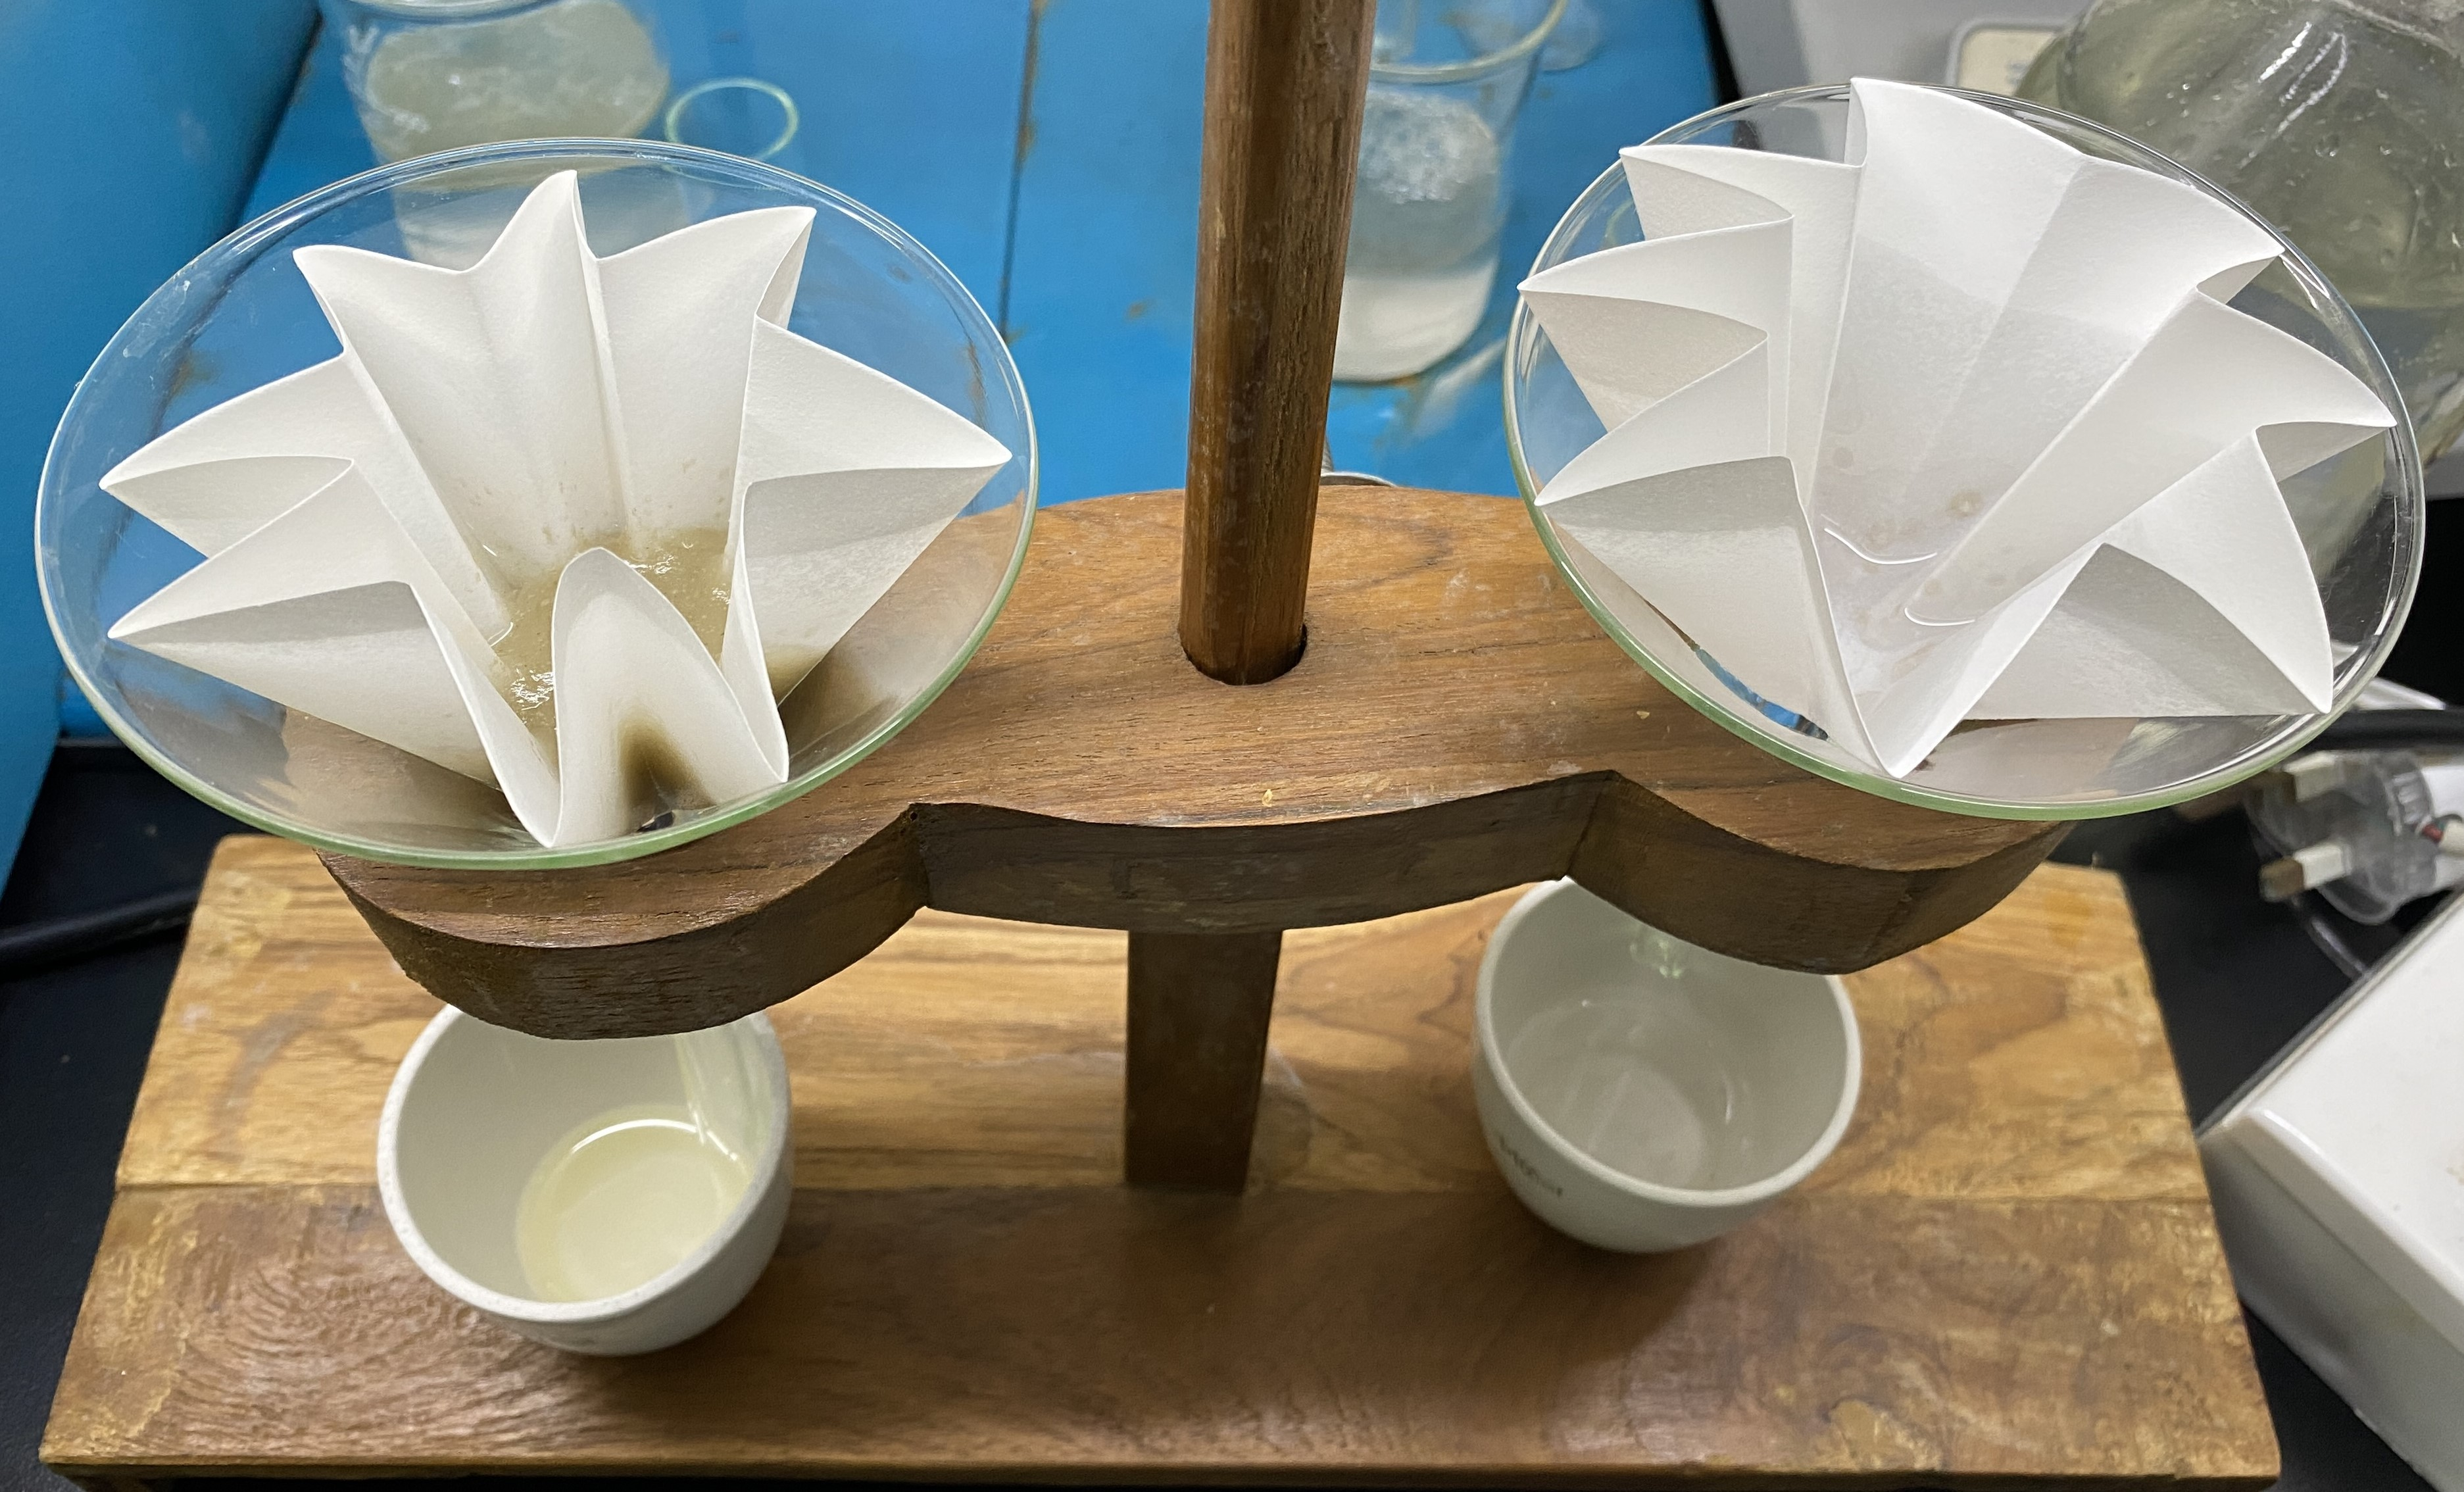
\includegraphics[width=.65\textwidth]{results/filtering_hexane_sample.JPG}\hfill


\caption{Photographs captured during the analysing of the \ac{OG} of inlet and outlet samples}
\label{fig: oil_and_grease_analyze_samples}
\end{figure}

\begin{figure}[H]
\centering

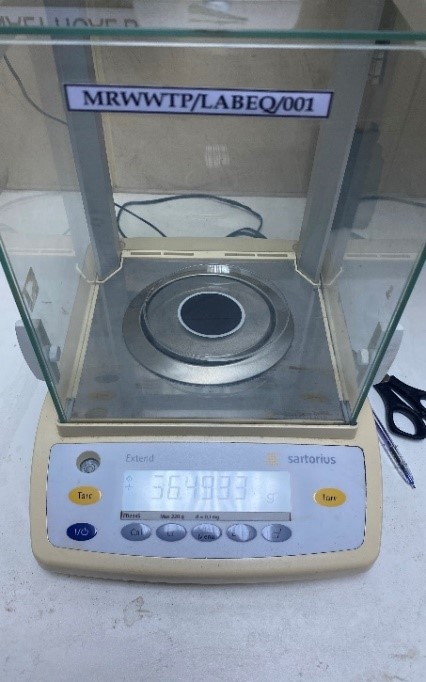
\includegraphics[width=.4\textwidth]{results/TSS.JPG}\hfill
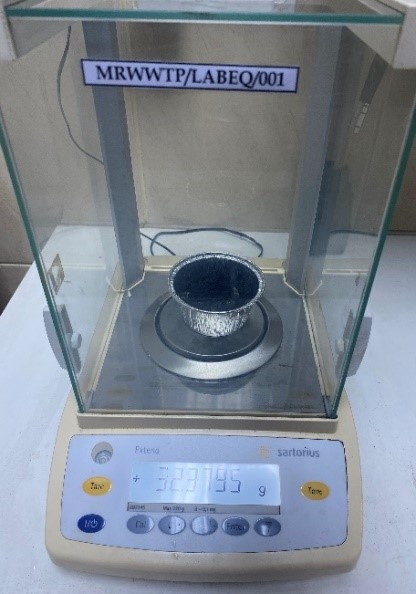
\includegraphics[width=.45\textwidth]{results/Dewatered sludge.jpg}\hfill

\caption{Measured weight of filtered paper for \ac{TSS} of the storage tank and the dried sludge sample }
\label{fig: TSS and Moisture content}
\end{figure}


\begin{figure}[H]
\centering
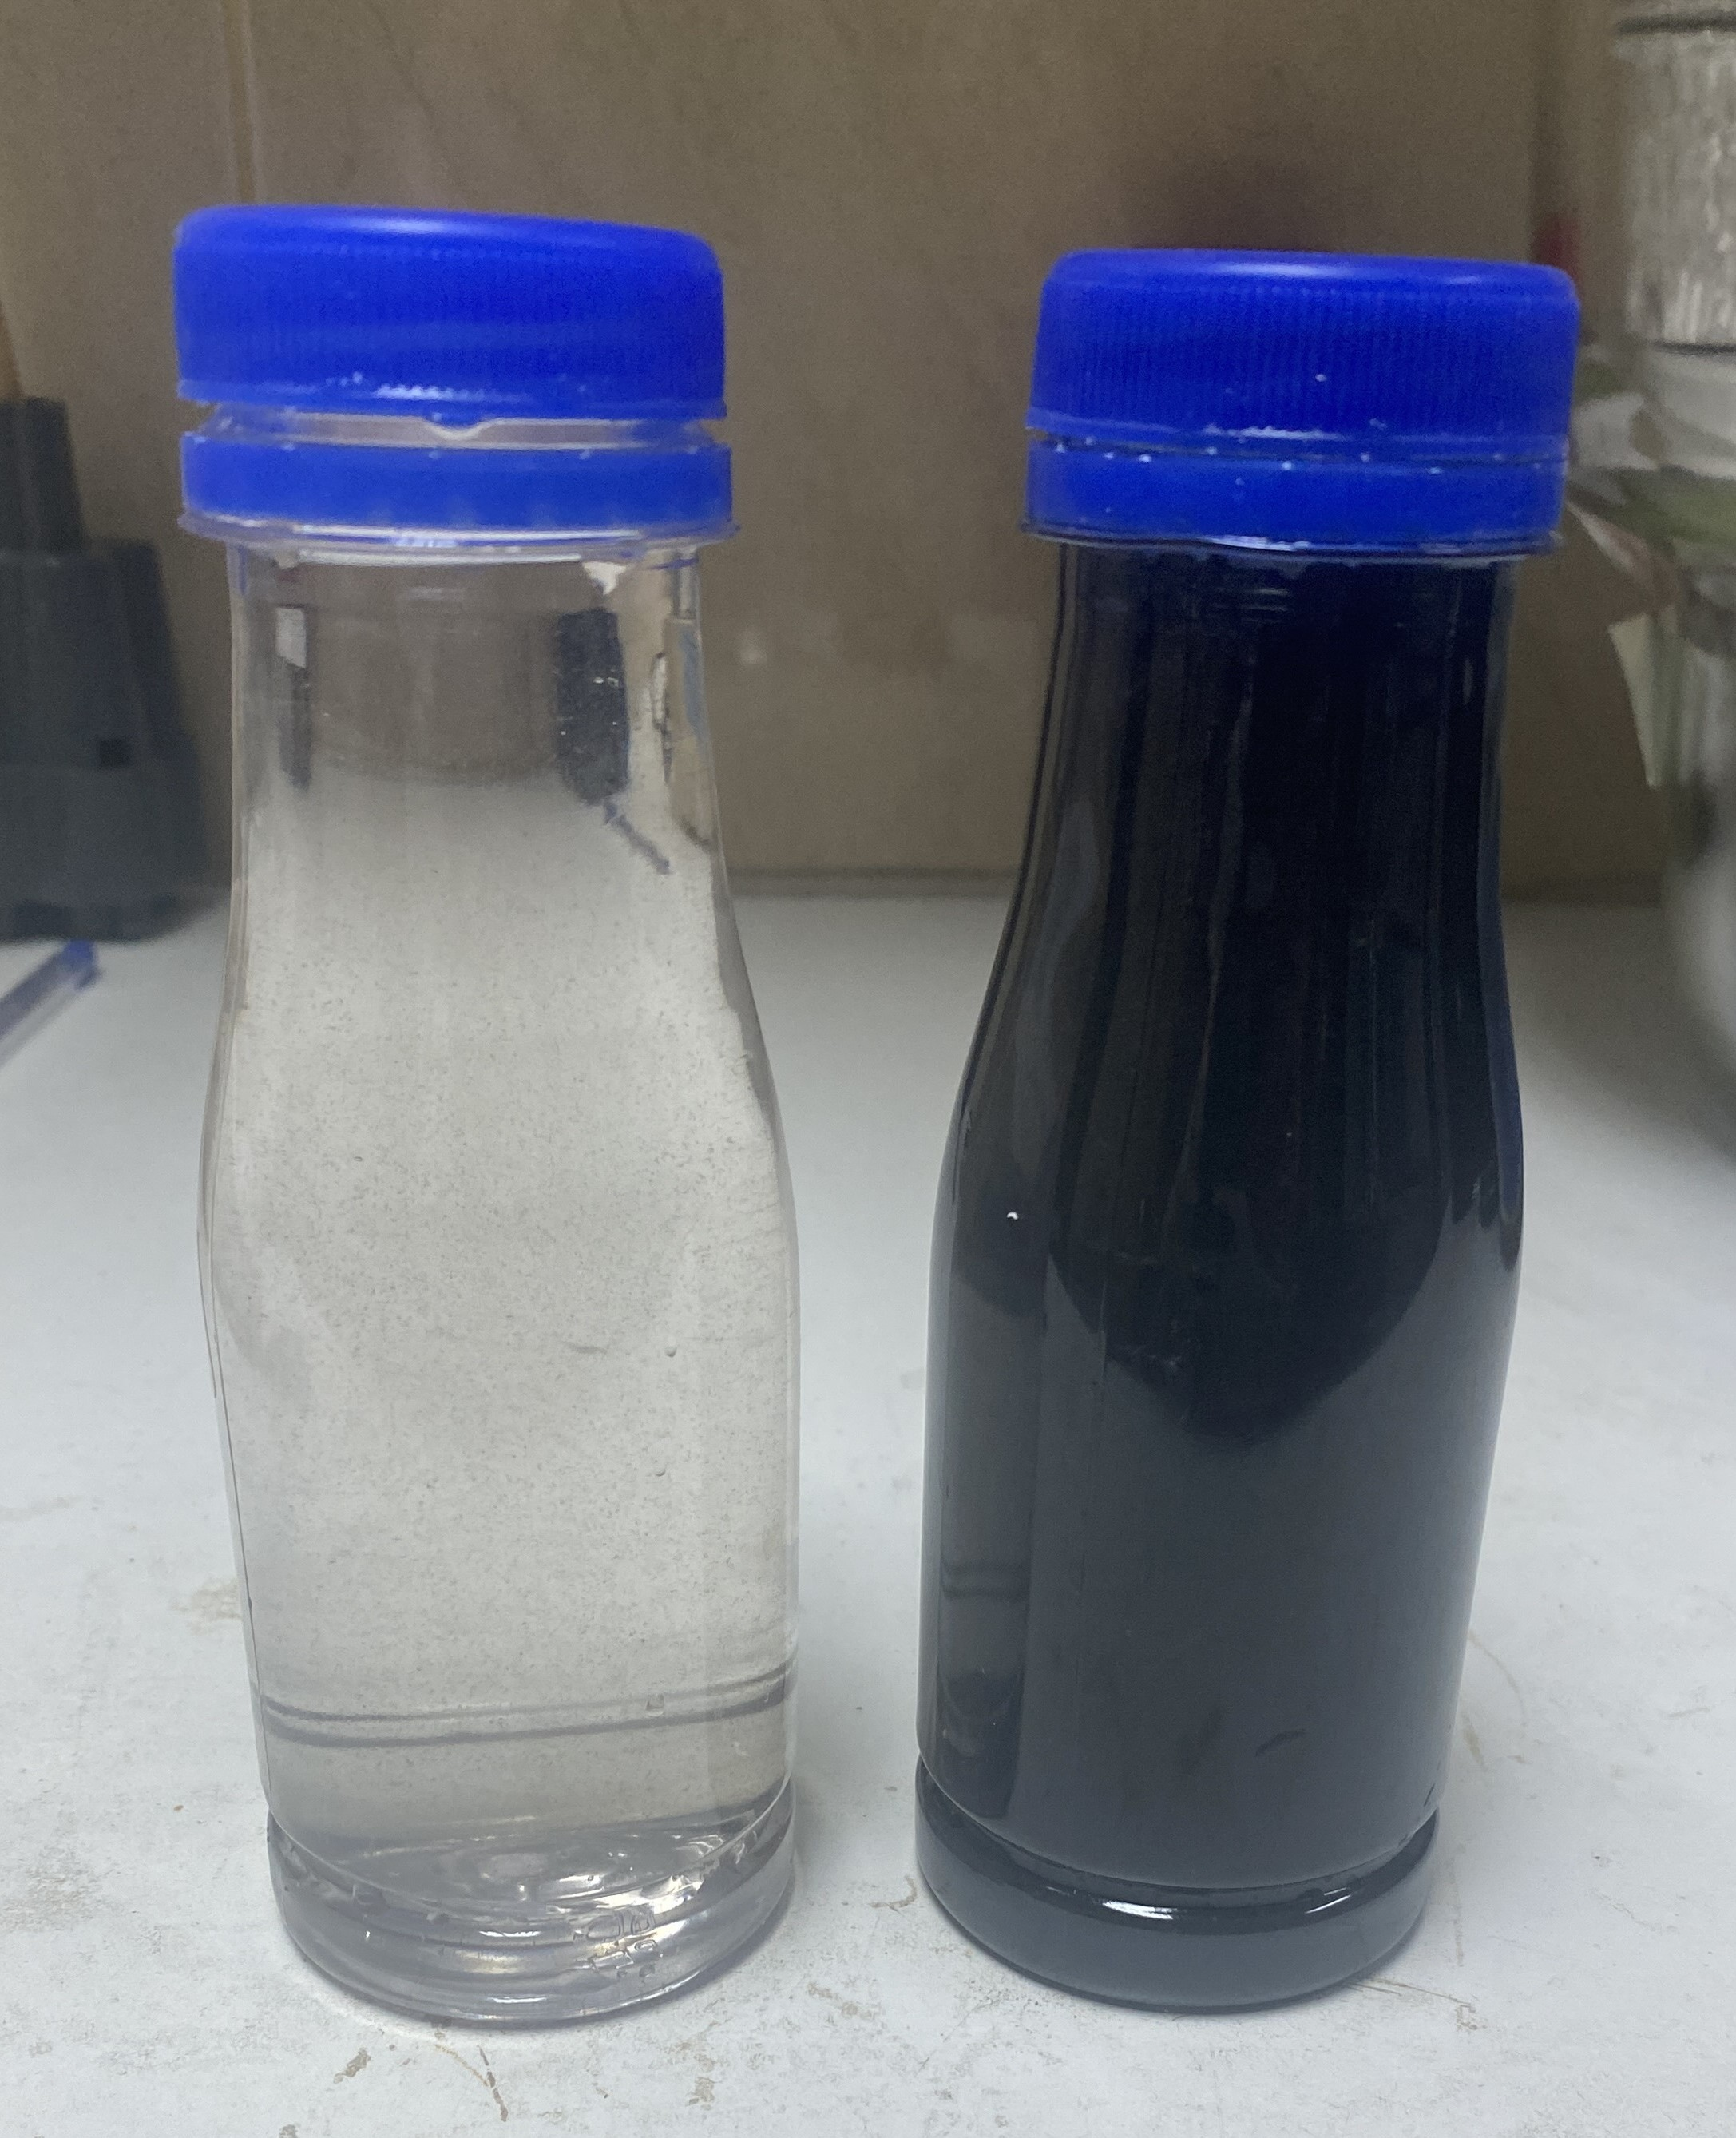
\includegraphics[width=0.4\linewidth]{results/Sample storage tank and return water.jpg}
\caption{Samples collected from the return water of the beltpress and the sludge storage tank}
\label{fig:Sample_storagetank_returnwater}
\end{figure}

\begin{figure}[H]
\centering
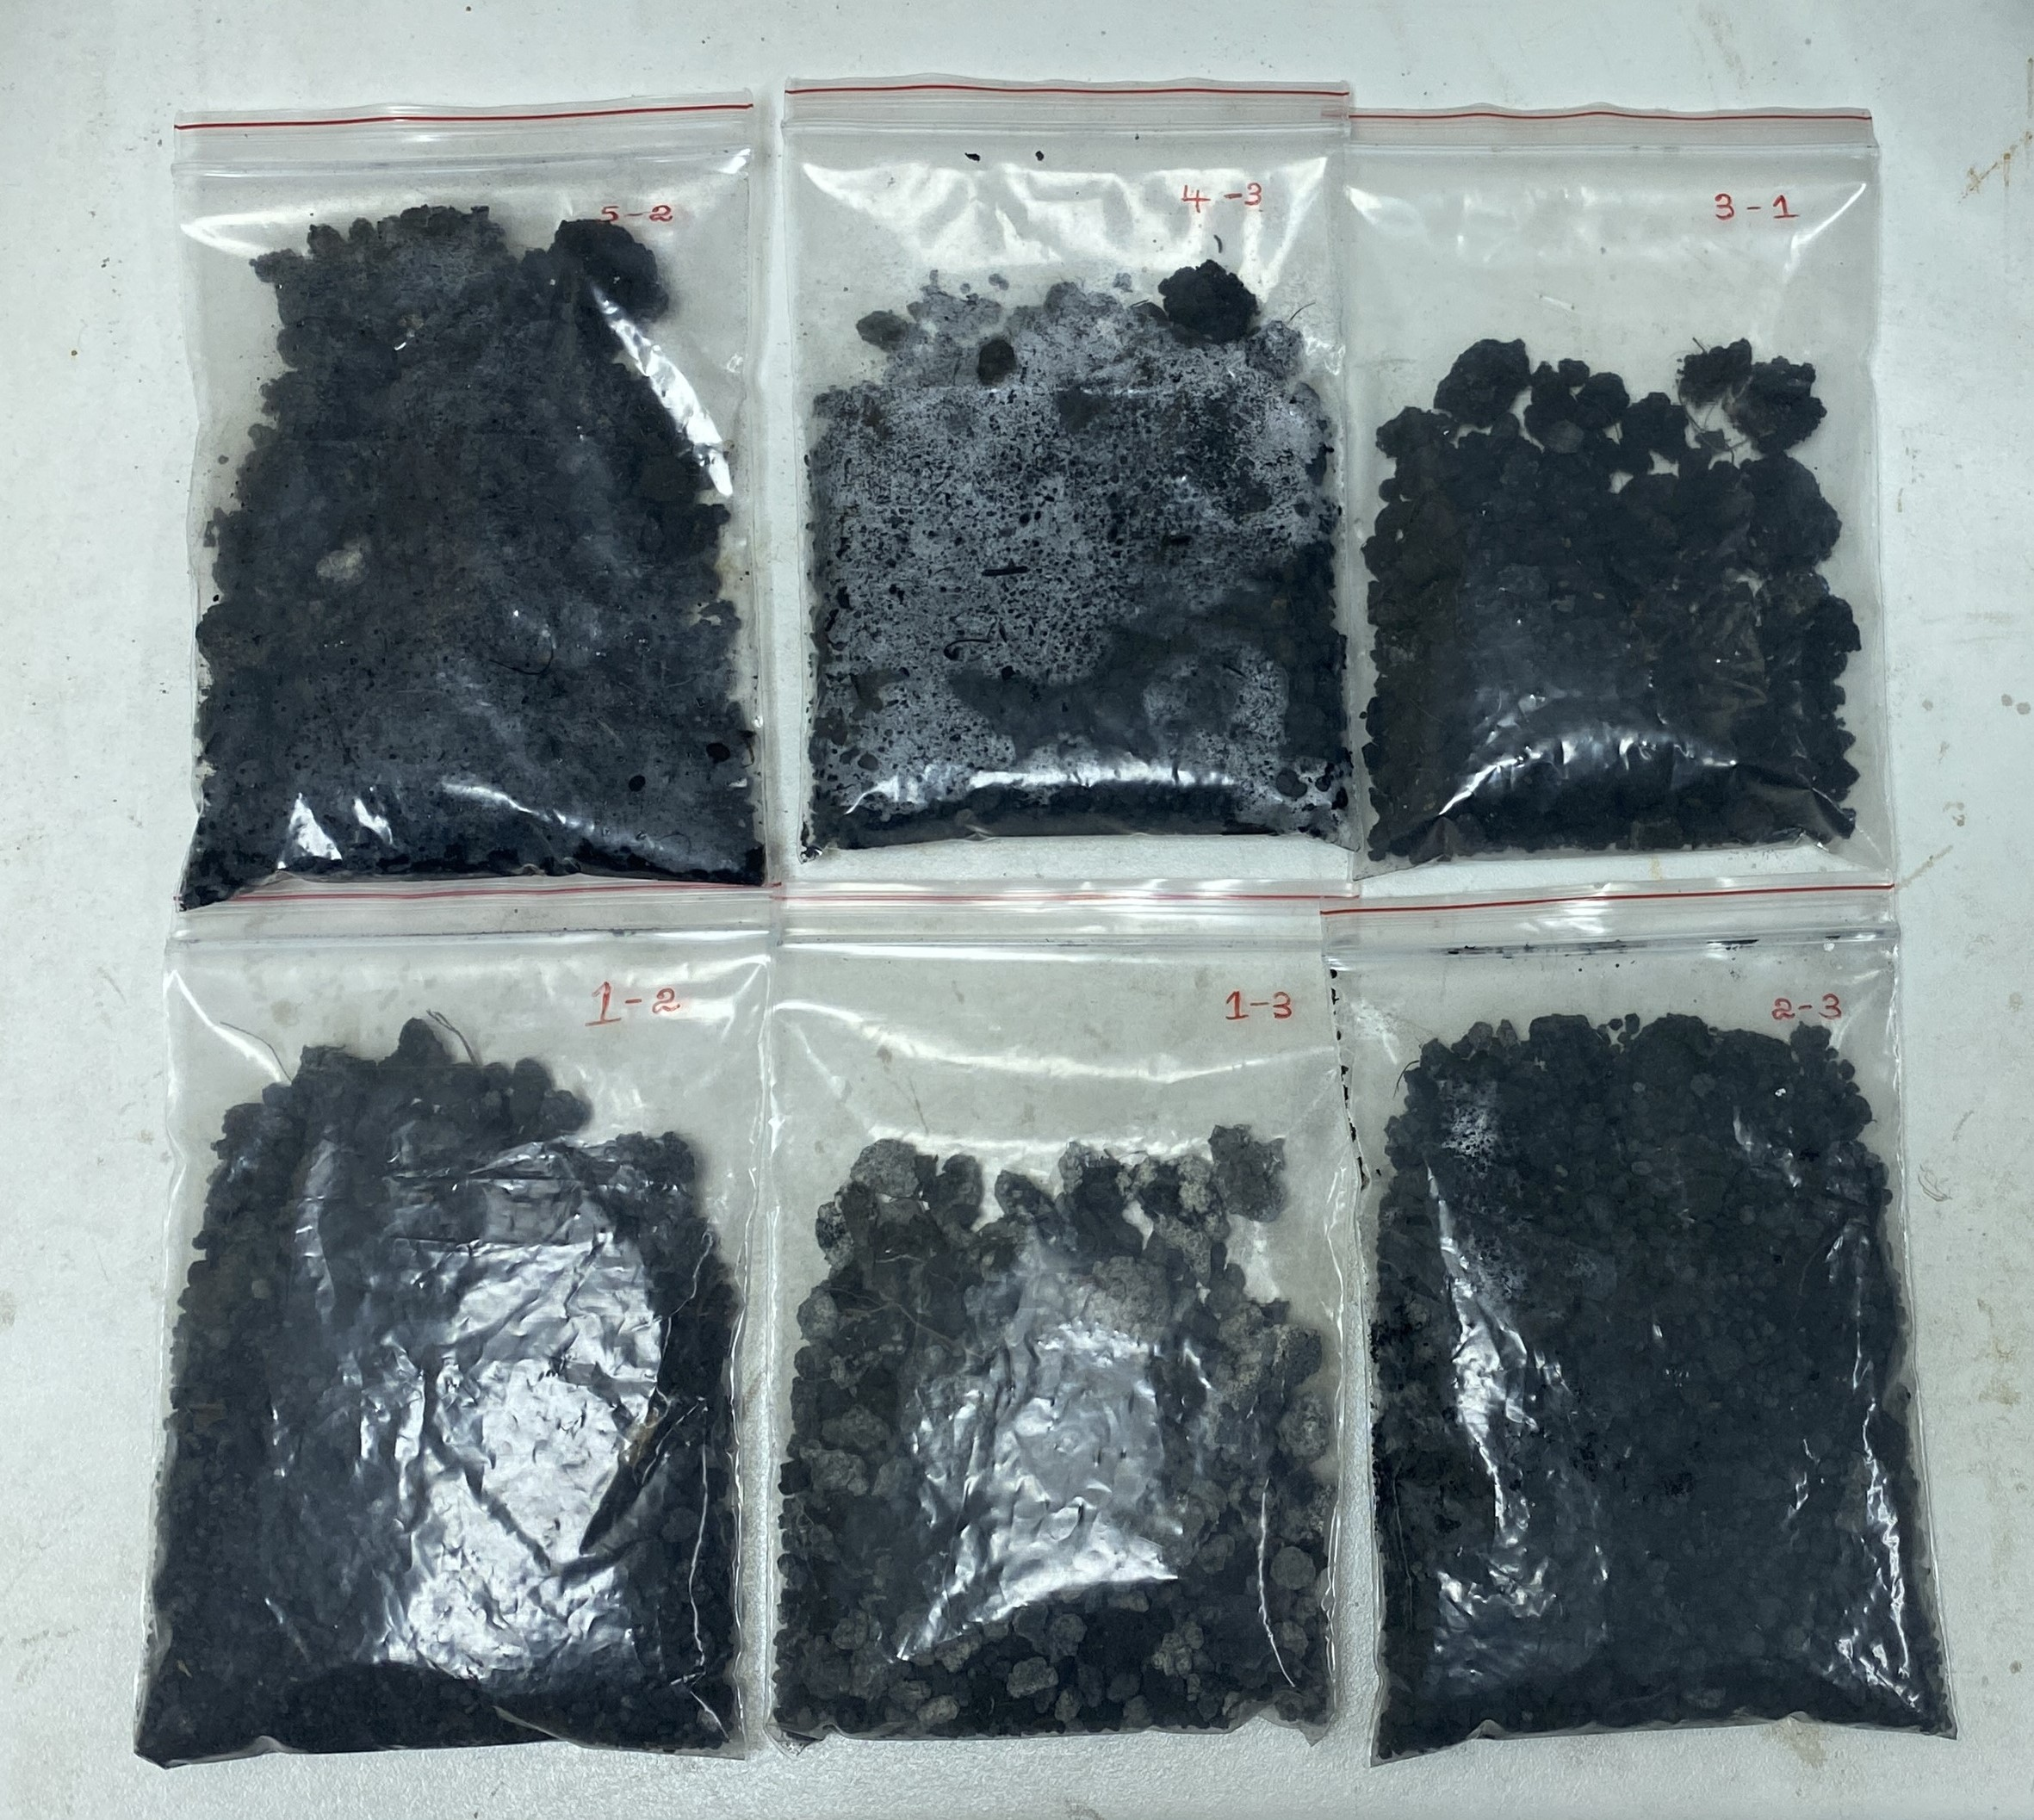
\includegraphics[width=0.6\linewidth]{results/Sample drying bed.jpg}
\caption{Samples ($S_4$) collected from the different sample points at the drying bed}
\label{fig:Sample_dryingbed}
\end{figure}


\newpage
\subsection{Characteristics of wastewater}

\subsubsection{Daily Flow}
During the study period, the flow remained relatively stable, fluctuating between \numprint{13000} and \numprint{18000} \unit{m^3} from sampling days 1 to 13. After that, between sample numbers 13 and 20, a notable increase in the flow was observed, ranging from \numprint{15000} to \numprint{37000} \unit{m^3}. After sampling day 20, the flow was stabilized again, with a variation between \numprint{7000} and \numprint{18000} \unit{m^3}. The highest flow was observed to be \numprint{36722} \unit{m^3} on sampling day 16, and the lowest flow was observed to be \numprint{7224} \unit{m^3} on sampling day 30. The average flow during the period was recorded to be \numprint{16671} \unit{m^3}.


\begin{figure}[H]
    \centering

    \pgfplotstableread[col sep=comma]{results/flow_dataset.csv} \dataset

    \begin{tikzpicture}
        \begin{axis}[
            axis lines = left,
            scaled ticks=false,
            xlabel = Week,
            width = 13cm,
            height = 10cm,
            ylabel = Flow \unit{m^3},
            legend pos = south west,
            ymax=40000,
            ymin=5000,
            ymajorgrids=true, % Display only major gridlines
            yminorgrids=true, % Display minor gridlines
            extra y tick labels={}, % Empty labels for extra y ticks
            extra y ticks={7500,12500,17500,22500,27500,32500,37500}, % Add extra y ticks with minor tick values
            extra y tick style={grid=minor, grid style={dashed,gray!50}}, % Style for extra y ticks
        ]

            \addplot table[x index = {0}, y index = {1}]{\dataset};
        \end{axis}
         \draw [thick, black] (-2.5,-1.75) rectangle (13,9);
    \end{tikzpicture}

    \caption{Variation of the flow}
    \label{fig:flow_graph}
\end{figure}

\subsubsection{Temperature}
A slight difference in the temperature between the influent and effluent was demonstrated, as shown in \Cref{fig:tempreature_graph}. For several samples, except for sample numbers 4, 16, 20, 25, and 30, a higher temperature was observed in the effluent than that of the influent. For sample number 23, the temperature values of the influent and the effluent water were equal. For sample number 16, the lowest temperature recorded for both the influent and effluent was 25.8 ℃ and 25.7 ℃, while the highest temperature recorded was 31.4 ℃ and 31.8 ℃, respectively, for sample number 12.

\begin{figure}[H]
\centering

\pgfplotstableread[col sep=comma]{results/temp_vs_time_dataset.csv} \dataset

\begin{tikzpicture} \begin{axis}[
    ybar = 1.5pt,
    bar width = 4pt,
    width = 15cm,
    height = 10cm,
    axis lines = left,
    enlarge x limits = 0.02,
    ymin = 25, ymax = 32,
    ymajorgrids=true, % Display only major gridlines
                    yminorgrids=true, % Display minor gridlines
                    extra y tick labels={}, % Empty labels for extra y ticks
                    extra y ticks={25.5,26.5, ..., 31.5}, % Add extra y ticks with minor tick values
                    extra y tick style={grid=minor, grid style={dashed,gray!50}}, % Style for extra y ticks
    legend style={at={(0.5,-0.15)},
    anchor=north,legend columns=-1},
    xlabel = Sample Number,
    ylabel = Temperature (°C),
]
    \addplot table[x index = {0}, y index = {1}]{\dataset};
    \addplot table[x index = {0}, y index = {2}]{\dataset};
    
    \legend{Influent, Effluent}
\end{axis}
\draw [thick, black] (-2,-2.25) rectangle (14,9);
\end{tikzpicture}

\caption{Variation in temperature of influent and effluent}
\label{fig:tempreature_graph}
\end{figure}

\subsubsection{Hydrogen ion concentration (pH)}
A slight variation in the pH between the influent and effluent was shown in \Cref{fig:ph_graph}. A pH range from 6.7 to 7.6 was exhibited for the influent, while a pH range from 6.8 to 7.7 was exhibited for the effluent. 
Higher values than 7 were indicated by the influent pH during the study period, except for sample numbers 14, 15, 16, 18, and 29, and higher values than sample number 7 were indicated by the effluent, except for sample numbers 18, 24, and 29. The lowest and highest pH values for influent and effluent were noted as 6.7 for sample number 29, 6.8 for sample number 18, 7.6 for sample number 3, and 7.7 for sample number 6, respectively. During the period, there were 15 samples where the pH value of the effluent was higher than that of the influent. The tolerance limit for the short sea outfall, outlined as 5.5 - 9.0, had not been exceeded by the effluent \cite{CEA2022}.


\begin{figure}[H]
\centering

\pgfplotstableread[col sep=comma]{results/ph_dataset.csv} \dataset

\begin{tikzpicture} \begin{axis}[
    ybar = 1.5pt,
    bar width = 4pt,
    width = 15cm,
    height = 10cm,
    axis lines = left,
    enlarge x limits = 0.02,
    ymin = 6.6,
    ymax = 7.8,
     ymajorgrids=true, % Display only major gridlines
                    yminorgrids=true, % Display minor gridlines
                    extra y tick labels={}, % Empty labels for extra y ticks
                    extra y ticks={6.7,6.9, ..., 7.7}, % Add extra y ticks with minor tick values
                    extra y tick style={grid=minor, grid style={dashed,gray!50}}, % Style for extra y ticks
    legend style={at={(0.5,-0.15)},
    anchor=north,legend columns=-1},
    xlabel = Week,
    ylabel = pH,
]
    \addplot table[x index = {0}, y index = {1}]{\dataset};
    \addplot table[x index = {0}, y index = {2}]{\dataset};
    
    \legend{Influent, Effluent}
\end{axis}
\draw [thick, black] (-2.25,-2.25) rectangle (14.25,9);
\end{tikzpicture}

\caption{Variation in pH of influent and effluent}
\label{fig:ph_graph}
\end{figure}

\subsubsection{Biochemical Oxygen Demand (BOD$_5$)}
Sewage \ac{BOD} refers to the quantity of oxygen required for the biochemical degradation of biodegradable organic substances in aerobic conditions. The amount of oxygen absorbed during the cycle is directly correlated to the quantity of decomposable organic matter \cite{Prasad2020}. A large variation in \ac{BOD5} between the influent and the effluent was shown in \Cref{fig:bod_graph}. The \ac{BOD5} levels for the influent and the effluent were varied between 32 and 456 mg/l and 3 and 18 mg/l, respectively. 

The highest value of 456 mg/l for the influent \ac{BOD5} was reported for sample number 19, and the lowest value of 32 mg/l was reported for sample number 8. The lowest \ac{BOD5} level for influent and the highest \ac{BOD5} level for effluent were shown in sample number 8. During this study period, the tolerance limit for the short sea outfall outlined as 75 mg/l has not been exceeded by the effluent \ac{BOD5} concentration \cite{CEA2022}. The influent concentration of \ac{BOD5} for sample numbers 8, 16, and 21 was measured lower than the tolerance limit for the shortsea outfall outlined. The removal efficiency of \ac{BOD5} was varied from 43.75\% to 98.68\%, and the average removal efficiency was calculated as 93.55\%. During the performance evaluation conducted in 2016, the removal efficiency of \ac{BOD5} was reported as 94.12\% \cite{Danushika2016}.

\begin{figure}[H]
\centering

\pgfplotstableread[col sep=comma]{results/bod_dataset.csv} \dataset

\begin{tikzpicture} \begin{axis}[
    ybar = 1.5pt,
    bar width = 5pt,
    width = 15cm,
    height = 10cm,
    axis lines = left,
    enlarge x limits = 0.02,
    ymin = 0,
    ymax = 500,
     ymajorgrids=true, % Display only major gridlines
                    yminorgrids=true, % Display minor gridlines
                    extra y tick labels={}, % Empty labels for extra y ticks
                    extra y ticks={50,150, ...,450}, % Add extra y ticks with minor tick values
                    extra y tick style={grid=minor, grid style={dashed,gray!50}}, % Style for extra y ticks
    legend style={at={(0.5,-0.15)},
    anchor=north,legend columns=-1},
    xlabel = Week,
    ylabel = BOD (mg/l),
]
    \addplot table[x index = {0}, y index = {1}]{\dataset};
    \addplot table[x index = {0}, y index = {2}]{\dataset};
    
    \legend{Influent, Effluent}
\end{axis}
\draw [thick, black] (-2.25,-2.25) rectangle (14.25,9);
\end{tikzpicture}

\caption{Variation in BOD$_{5}$ of influent and effluent}
\label{fig:bod_graph}
\end{figure}


\subsubsection{Chemical Oxygen Demand (COD)}
\ac{COD} is the quantity of oxygen required for the oxidation of organic and some inorganic matter \cite{Prasad2020}, and there was a large variation in \ac{COD} between the influent and the effluent. The \ac{COD} levels for the influent and the effluent varied from 169 to 1647 mg/l and 23 to 76 mg/l, respectively. The \ac{COD} concentration of the influent for the first nine samples was shown below 600 mg/l and was increased sharply for sample number 10. However, for sample number 11, \ac{COD} concentration was decreased sharply and again showed a sharp increase for sample number 12. For sample numbers 13 to 15, an increasing trend was visible, with a sharp drop for sample numbers 15 to 16. For sample number 19, the \ac{COD} concentration was indicated as its highest value for the period. Between sample numbers 19, and 21, \ac{COD} indicated a sharp decrease. A gradual increment from sample number 25 to 27 and a sharp decrease from sample number 27 to 29 were noted. During this study period, the effluent \ac{COD} concentration did not exceed the tolerance limit of 400 mg/l \cite{CEA2022}. The influent \ac{COD} concentration was below the tolerance limit of effluent for short sea outfall for 15 samples, and the removal efficiencies varied from 63.29\% to 97.21\% during this period. The average \ac{COD} removal efficiency was reported as 86.95\%, and the \ac{COD} removal efficiency reported during the performance evaluation done in 2016 was 88.52\% \cite{Danushika2016}.

\begin{figure}[H]
\centering

\pgfplotstableread[col sep=comma]{results/cod_dataset.csv} \dataset

\begin{tikzpicture} \begin{axis}[
    ybar = 1.5pt,
    bar width = 5pt,
    width = 15cm,
    height = 10cm,
    axis lines = left,
    enlarge x limits = 0.02,
    ymin = 0,
    ymax = 1700,
     ymajorgrids=true, % Display only major gridlines
                    yminorgrids=true, % Display minor gridlines
                    extra y tick labels={}, % Empty labels for extra y ticks
                    extra y ticks={100,300, ..., 1700}, % Add extra y ticks with minor tick values
                    extra y tick style={grid=minor, grid style={dashed,gray!50}}, % Style for extra y ticks
    legend style={at={(0.5,-0.15)},
    anchor=north,legend columns=-1},
    xlabel = Week,
    ylabel = COD (mg/l),
]
    \addplot table[x index = {0}, y index = {1}]{\dataset};
    \addplot table[x index = {0}, y index = {2}]{\dataset};
    
    \legend{Influent, Effluent}
\end{axis}
\draw [thick, black] (-2.25,-2.25) rectangle (14.25,9);
\end{tikzpicture}

\caption{Variation of COD of influent and effluent }
\label{fig:COD_graph}
\end{figure}


\subsubsection{Total Suspended Solids (TSS)}
\Cref{fig:tss_graph} shows a slight variation in \ac{TSS} between the influent and the effluent during this period. The influent and effluent concentrations of \ac{TSS} were varied from 74 to 1438 mg/l and 4 to 28 mg/l, respectively. The highest and lowest concentrations of influent \ac{TSS} were observed in sample numbers 19, and 21. The concentrations of \ac{TSS} observed for the first 9 samples were indicated as values below 450 mg/l, and after sample number 10, a sharp increase in the influent \ac{TSS} concentration was observed.

From sample numbers 10 to 19, the influent \ac{TSS} concentration fluctuated, and in sample 19, \ac{TSS} concentration reached its peak, followed by a sharp decrease in the next two samples. For the last nine samples, the \ac{TSS} concentration did not exceed 700 mg/l. For samples 6, 20, and 24, the lowest effluent concentration of \ac{TSS} was observed, and in sample 9, the highest value for the effluent \ac{TSS} was reported. During this study period, the effluent \ac{TSS} concentration did not exceed the tolerance limit of 50 mg/l \cite{CEA2022}. The removal efficiencies for this period varied from 75.44\% to 99.32\%, and the average removal efficiency was found to be 95.28\%. However, during the performance evaluation conducted in 2016, the removal efficiency of \ac{TSS} was reported as 97.05\% \cite{Danushika2016}.

\begin{figure}[H]
\centering

\pgfplotstableread[col sep=comma]{results/tss_dataset.csv} \dataset

\begin{tikzpicture} \begin{axis}[
    ybar = 1.5pt,
    bar width = 5pt,
    width = 15cm,
    height = 10cm,
    axis lines = left,
    enlarge x limits = 0.02,
    ymin = 0,
    ymax = 1500,
    ymajorgrids=true, % Display only major gridlines
                    yminorgrids=true, % Display minor gridlines
                    extra y tick labels={}, % Empty labels for extra y ticks
                    extra y ticks={100,300, ..., 1500}, % Add extra y ticks with minor tick values
                    extra y tick style={grid=minor, grid style={dashed,gray!50}}, % Style for extra y ticks
    legend style={at={(0.5,-0.15)},
    anchor=north,legend columns=-1},
    xlabel = Week,
    ylabel = TSS (mg/l),
]
    \addplot table[x index = {0}, y index = {1}]{\dataset};
    \addplot table[x index = {0}, y index = {2}]{\dataset};
    
    \legend{Influent, Effluent}
\end{axis}
\draw [thick, black] (-2.25,-2.25) rectangle (14.25,9);
\end{tikzpicture}

\caption{Variation in TSS of influent and effluent}
\label{fig:tss_graph}
\end{figure}




\subsubsection{Oil and Grease Concentration}

One common type of pollutant found in water and wastewater is "oil and grease." Organic compounds of the \ac{OG} group have an extremely low affinity for water. Substances commonly categorized as consists of hydrocarbons, soaps, fatty acids, waxes, and lipids \cite{Pintor2016}. A large variation between the influent and the effluent was shown in \ac{OG} concentration in \Cref{fig:OG_graph}. The variation of the \ac{OG} in the influent and the effluent was observed to be 7.5 to 26.8 mg/l and 0 to 1.1 mg/l, respectively. In several samples, the influent \ac{OG} concentration was higher than 10 mg/l, and the average concentration was 15.16 mg/l. In the first 5 samples, concentration varied between 10 and 15 mg/l, and after that, a sharp increase was noted in sample number 6.

From sample numbers 6 to 9, the concentration of \ac{OG} varied between 15 and 25 mg/l. The highest and lowest concentrations of influent were observed in sample numbers 14 and 21. An equal concentration was shown in both samples 16 and 17 as 12.5 mg/l. The concentration of effluent did not exceed the tolerance limit for shortsea outfall outlined as 12 mg/l, and for sample number 8, the \ac{OG} concentration of influent too was indicated to be lower than the tolerance limit \cite{CEA2022}. The removal efficiency of the \ac{OG} was found to be 97.04\%.\\

\begin{figure}[H]
\centering

\pgfplotstableread[col sep=comma]{results/oil_and_grease_dataset.csv} \dataset

\begin{tikzpicture} \begin{axis}[
    ybar = 1.5pt,
    bar width = 5pt,
    width = 15cm,
    height = 10cm,
    axis lines = left,
    enlarge x limits = 0.03,
    ymin = 0,
    ymajorgrids=true, % Display only major gridlines
                    yminorgrids=true, % Display minor gridlines
                    extra y tick labels={}, % Empty labels for extra y ticks
                    extra y ticks={2.5,7.5,12.5,17.5,22.5}, % Add extra y ticks with minor tick values
                    extra y tick style={grid=minor, grid style={dashed,gray!50}}, % Style for extra y ticks
    legend style={at={(0.5,-0.15)},
    anchor=north,legend columns=-1},
    xlabel = Week,
    ylabel = Oil \& Grease (mg/l),
]
    \addplot table[x index = {0}, y index = {1}]{\dataset};
    \addplot table[x index = {0}, y index = {2}]{\dataset};
    
    \legend{Influent, Effluent}
\end{axis}
\draw [thick, black] (-2,-2.25) rectangle (14,9);
\end{tikzpicture}

\caption{Variation of Oil and Grease}
\label{fig:OG_graph}
\end{figure}


\subsubsection{Ortho Phosphate (as P)}
During the study period, as depicted in \Cref{fig:OrthoP_graph}, several samples showed that the concentration of orthophosphate was more than 0.4 mg/l. The highest observed orthophosphate concentration of the influent was noted as 0.8 mg/l for sample numbers 10, 22, and 30, and the lowest orthophosphate concentration of the influent was noted as 0.1 mg/l in sample 17. For the first nine samples, the concentration varied between 0.4 and 0.8 mg/l, and after sample 13, the concentration of influent was decreased to 0.2 mg/l.

From sample numbers 14 to 18, the concentration of influent varied from 0.1 to 0.3 mg/l, while the last 12 samples, starting from sample number 19, showed that the influent orthophosphate concentration lied between 0.4 and 0.8 mg/l. Considering the effluent orthophosphate concentration, the samples from 5 to 8 showed equal values, and since then, there has been a gradual increase between sample numbers 8 and 10. A sharp decrease in concentration was observed between sample numbers 10 and 11. From sample numbers 11 to 30, the concentration was observed below 0.2 mg/l, and during the study period, the orthophosphate concentration of both the influent and effluent did not exceed the tolerance limit for short sea outfall outlined as 5.0 mg/l \cite{CEA2022}. 
\begin{figure}[H]
\centering

\pgfplotstableread[col sep=comma]{results/ortho_posphate_dataset.csv} \dataset

\begin{tikzpicture} \begin{axis}[
    ybar = 1.5pt,
    bar width = 5pt,
    width = 15cm,
    height = 10cm,
    axis lines = left,
    enlarge x limits = 0.03,
    ymin = 0,
    ymajorgrids=true, % Display only major gridlines
                    yminorgrids=true, % Display minor gridlines
                    extra y tick labels={}, % Empty labels for extra y ticks
                    extra y ticks={0.15, 0.25,0.35,0.45,0.55,0.65,0.75}, % Add extra y ticks with minor tick values
                    extra y tick style={grid=minor, grid style={dashed,gray!50}}, % Style for extra y ticks
    legend style={at={(0.5,-0.15)},
    anchor=north,legend columns=-1},
    xlabel = Week,
    ylabel = Ortho Posphate (\unit{mg/l}),
]
    \addplot table[x index = {0}, y index = {1}]{\dataset};
    \addplot table[x index = {0}, y index = {2}]{\dataset};
    
    \legend{Influent, Effluent}
\end{axis}
\draw [thick, black] (-2,-2.25) rectangle (14,9);
\end{tikzpicture}

\caption{Variation of Ortho Phosphate of influent and effluent }
\label{fig:OrthoP_graph}
\end{figure}




\subsubsection{Fluoride (as F)}
\Cref{fig:Fluo_graph} shows a considerable variation in the concentration of fluoride (as F) in the influent and the effluent. For the first four samples, the influent concentration was reported below 0.3 mg/l, while the lowest concentration of 0.2 mg/l was observed in samples 16, 17, and 19. Thereafter, the concentration of fluoride in the influent was noted as 0.5 mg/l, and a gradual decrease between sample numbers 20 and 22 was observed.

For sample numbers 23 and 24, the concentration was indicated as 0.4 mg/l, and then a gradual increase was observed from sample 24. The concentration of the influent was indicated as 0.6 mg/l for both sample numbers 26 and 27, and a decreasing trend was visible from samples 27 to 29. The highest concentration of the influent, 0.7 mg/l, was observed during the last sample of the study period. The fluoride concentration of the effluent showed values less than or equal to 0.2 mg/l during the study period. Importantly, both influent and effluent concentrations did not exceed the tolerance limit outlined as 2 mg/l \cite{CEA2022}.


\begin{figure}[H]
\centering

\pgfplotstableread[col sep=comma]{results/fluoride_dataset.csv} \dataset
\begin{tikzpicture} \begin{axis}[
    ybar = 2pt,
    bar width = 5pt,
    width = 15cm,
    height = 10cm,
    axis lines = left,
    % enlargelimits=0.01,
    xmax = 31,
    xmin = 15,
    ymin = 0.05,
    ymajorgrids=true, % Display only major gridlines
                    yminorgrids=true, % Display minor gridlines
                    extra y tick labels={}, % Empty labels for extra y ticks
                    extra y ticks={0.15, 0.25,0.35,0.45,0.55,0.65}, % Add extra y ticks with minor tick values
                    extra y tick style={grid=minor, grid style={dashed,gray!50}}, % Style for extra y ticks
    legend style={at={(0.5,-0.15)},
    anchor=north,legend columns=-1},
    ylabel = Fluoride (mg/l),
    xtick=data,
]
    \addplot table[x index = {0}, y index = {1}]{\dataset};
    \addplot table[x index = {0}, y index = {2}]{\dataset};
    \legend{Influent, Effluent}
\end{axis}
\draw [thick, black] (-2,-2.25) rectangle (14,9);
\end{tikzpicture}

\caption{Variation of Fluoride (as F) of influent and effluent }
\label{fig:Fluo_graph}
\end{figure}


\subsubsection{BOD/COD Ratio}
Biodegradability was calculated using the ratio of \ac{BOD5} and \ac{COD}, and as shown in \Cref{fig:BOD/COD_graph}, for the influent, the ratio between \ac{BOD5} and \ac{COD} lied between 0.18 and 0.56. The effluent \ac{BOD5}/\ac{COD} ratio ranged between 0.08 and 0.36. In the majority of samples, the \ac{BOD5}/ \ac{COD} ratio of the influent showed values below 0.50, except for samples 14 and 27. Considering the effluent, the \ac{BOD5}/\ac{COD} ratio was below 0.30 most of the time, except for sample numbers 8, 10, 14, and 28. The highest and lowest ratios were calculated as 0.56 in sample 14 and 0.18 in sample 8, respectively. The average value of the ratio was observed as 0.39 for the influent. The highest and lowest values were observed for the effluent, which was 0.36 in sample 8 and 0.08 in sample 6, with an average of 0.18. 
\begin{figure}[H]
\centering

\pgfplotstableread[col sep=comma]{results/bod_cod_ratio_dataset.csv} \dataset

\begin{tikzpicture} \begin{axis}[
    ybar = 1.5pt,
    bar width = 4pt,
    width = 15cm,
    height = 10cm,
    axis lines = left,
    enlarge x limits = 0.02,
    ymin = 25, ymax = 32,
    legend style={at={(0.5,-0.15)},
    anchor=north,legend columns=-1},
    xlabel = Sample Number,
    ylabel = BOD$_5$ / COD,
    ymax=0.6, ymin=0,
    ymajorgrids=true, % Display only major gridlines
                    yminorgrids=true, % Display minor gridlines
                    extra y tick labels={}, % Empty labels for extra y ticks
                    extra y ticks={0.15, 0.25,0.35,0.45,0.55}, % Add extra y ticks with minor tick values
                    extra y tick style={grid=minor, grid style={dashed,gray!50}}, % Style for extra y ticks
]
    \addplot table[x index = {0}, y index = {1}]{\dataset};
    \addplot table[x index = {0}, y index = {2}]{\dataset};
    
    \legend{Influent, Effluent}
\end{axis}
\draw [thick, black] (-2,-2.25) rectangle (14,9);
\end{tikzpicture}

\caption{Variation in biodegradability of influent and effluent}
\label{fig:BOD/COD_graph}
\end{figure}



\subsection{Removal Efficiencies}
According to \Cref{tab:average_removal_efficiency_table}, the highest average \ac{BOD5} removal efficiency was indicated in November as 97.34\%, and the lowest efficiency was indicated as 82.49\% in July. There was an average efficiency during the period indicated as 93.55\%. The highest average \ac{COD} removal efficiency was indicated in July, and the lowest value was indicated in June during the study period. As shown in \Cref{tab:average_removal_efficiency_table}, the monthly average \ac{TSS} removal efficiencies vary from 91.46\% to 97.80\%. Moreover, the average removal efficiencies of \ac{OG}, orthophosphate, and fluoride were indicated as 97.04\%, 79.08\%, and 68.04\%, respectively. During this period, the orthophosphate and fluoride removal efficiencies increased gradually.

\begin{table}[H]
    \caption{Average removal efficiencies of different parameters}
    \begin{tabular}{|>{\raggedright\arraybackslash}p{0.135\linewidth}|>{\centering\arraybackslash}p{0.11\linewidth}|>{\centering\arraybackslash}p{0.11\linewidth}|>{\centering\arraybackslash}p{0.11\linewidth}|>{\centering\arraybackslash}p{0.11\linewidth}|>{\centering\arraybackslash}p{0.12\linewidth}|>{\centering\arraybackslash}p{0.105\linewidth}|}
        \hline
        \textbf{Month}     & \textbf{BOD$_5$  (\%)} & \textbf{COD (\%)}& \textbf{TSS (\%)} & \textbf{Oil \& Grease (\%)} & \textbf{Ortho-phosphate (\%)} & \textbf{Fluoride (as F) (\%)} \\
        \hline
        \textbf{June}      & 94.24                                                        & 95.78             & 96.73             & 95.78                  & -                        & -                        \\
        \textbf{July}      & 82.49                                                        & 98.36             & 91.46             & 98.36                  & 79.17                    & -                        \\
        \textbf{August}    & 94.56                                                        & 97.53             & 92.71             & 97.53                  & 73.50                    & -                        \\
        \textbf{September} & 96.04                                                        & 97.35             & 95.74             & 97.35                  & 67.50                    & 45.83                    \\
        \textbf{October}   & 94.43                                                        & 96.50             & 96.54             & 96.50                  & 88.27                    & 61.67                    \\
        \textbf{November}  & 97.34                                                        & 96.69             & 97.80             & 96.69                  & 82.00                    & 78.97                    \\
        \textbf{December}  & 92.37                                                        & 96.54             & 96.64             & 96.54                  & 85.48                    & 75.86                    \\
        \hline
        \hline
        \textbf{Min}       & 43.75                                                        & 63.29             & 75.44             & 94.20                  & 50.00                    & 45.83                    \\
        \textbf{Max}       & 98.68                                                        & 97.21             & 99.32             & 100.00                 & 92.59                    & 88.33                    \\
        \textbf{Average}   & 93.55                                                        & 86.95             & 95.28             & 97.04                  & 79.08                    & 68.04                    \\
        \textbf{SD}        &  9.91                                                            &  8.84                & 5.26                  &  1.38                       & 9.92                          &  14.80\\
     \hline
    \end{tabular}
    \label{tab:average_removal_efficiency_table}
\end{table}

\subsection{Correlation}
The consistency of correlations between different measures of organic content depends mostly on the characteristics of the wastewater and its origin. Regression analysis was used to assess the relationship between influent \ac{BOD5} and influent \ac{TSS}. Due to the rapidness of \ac{TSS} tests, these correlations can be highly beneficial, as \ac{BOD5} measurements require 5 days. After establishing the correlation, \ac{TSS} monitoring can be effectively utilized for treatment plant operation \cite{Kumar2010}.

\begin{table}[H]
    \centering
    
\caption{Correlation between \ac{BOD5} and \ac{TSS}}
\label{tab:BOD_TSS_correlations}
    \begin{tabular}{|>{\raggedright\arraybackslash}p{5cm}|>{\centering\arraybackslash}p{5cm}|>{\centering\arraybackslash}p{4.5cm}|}
    \hline
          & Expression & Correlation Coefficient \\
          \hline
         Variation between influent \ac{BOD5} (y) and \ac{TSS} (x) & $y = 47.8427 + 0.3925x$  & $ r = 0.8194$ \\
         \hline
    \end{tabular}
\end{table}


According to the \Cref{tab:BOD_TSS_correlations}, the correlation coefficient between \ac{TSS} and \ac{BOD5} was 0.8194, demonstrating a strong positive linear relationship between the two variables. The regression analysis demonstrated a statistically significant relationship between \ac{TSS} and \ac{BOD5}, with a p-value shown as $3.075 e{-8}$, less than 0.05, which concludes rejecting the null hypothesis (H0). In addition, the regression model demonstrated a good level of fit to the data, as seen by the higher value of the adjusted R-squared value of 0.6596, which indicates nearly 66\% of the variation of the data is explained by the fitted regression model in \ac{BOD5}. 

\begin{figure}[H]
\centering

\pgfplotstableread[col sep=comma]{results/measure_predicted_data.csv} \dataset
\begin{tikzpicture} \begin{axis}[
    width = 15cm,
    height = 10cm,
    axis lines = left,
    xlabel = Sample Number,
    % enlargelimits=0.01,
    xmax = 31,
    xmin = 9,
    ymin = 0,
    ymax = 500,
    ymajorgrids=true, % Display only major gridlines
                    yminorgrids=true, % Display minor gridlines
                    extra y tick labels={}, % Empty labels for extra y ticks
                    extra y ticks={50, 150,250,350,450}, % Add extra y ticks with minor tick values
                    extra y tick style={grid=minor, grid style={dashed,gray!50}}, % Style for extra y ticks
    legend style={at={(0.5,-0.15)},
    anchor=north,legend columns=-1},
    ylabel = $BOD_5$ (mg/l),
    xtick=data,
]
    \addplot table[x index = {0}, y index = {1}]{\dataset};
    \addplot table[x index = {0}, y index = {2}]{\dataset};
    \legend{measured, predicted}
\end{axis}
\draw [thick, black] (-2,-2.25) rectangle (14,9);
\end{tikzpicture}

\caption{Comparison between actual measured \ac{BOD5}  values  and  calculated \ac{BOD5} values using the regression equation}
\label{fig:measured_predicted_graph}
\end{figure}



\Cref{fig:measured_predicted_graph} shows the comparison between measured values and predicted values using a regression analysis equation with the last 20 data points from the approved dataset. The sample numbers are the same as mentioned in \Cref{table:sample_numbering}, and since it was identified as an outlier, sample number 19 was removed from the dataset. The largest variation is shown as 160 mg/l in sample number 14, and there are two samples with a higher difference between measured and predicted values of more than 100 mg/l. Furthermore, 4 samples show a difference of more than 60 to less than 100 mg/l between predicted and measured values. 



\newpage
\subsection{Sludge Management}

\subsubsection{Belt Filter Press Efficiency}
From December to February, the belt filter press efficiency was measured using the dry solid content of the dewatered sludge cake. During the time period, the dry solid content of the sludge cake varied from 11.00\% to 14.50\%. The highest dry solid content of 14.06\% was observed on $01^{st}$ December 2023, and the lowest dry solid content of 11.32\% was noted on $08^{th}$ January 2024.

The \ac{TSS} concentration of the sludge storage tank and the return water from the belt press are shown in \Cref{fig:Solid_Recovered_graph}. The sludge storage tank had a \ac{TSS} value between \numprint{20000} mg/l and \numprint{30000} mg/l. The return water \ac{TSS} concentration varies between 80 mg/l and 300 mg/l. The percentage of solid recovery is over 99\% for the study period.

\begin{figure}[H]
\centering

\pgfplotstableread[col sep=comma] {results/ds_content_dataset.csv} \dataset
                \begin{tikzpicture}
                \begin{axis}[
                ybar,
                bar width = 10pt,
                    date coordinates in=x,
                    axis lines = left,
                    table/col sep=comma,
                    xlabel = Date,
                    xlabel style={
                        at={(0.5,-11ex)}
                    },
                    xticklabel style={
                        rotate=45,
                        anchor=near xticklabel,
                    },
                    xtick=data,
                    xticklabel=\year-\month-\day,
                    width = 15cm,
                    height = 9cm,
                    ylabel = Solid Content (\%),
                    ymax=15,
                    ymin=10,
                     xmin = 2023-11-25,
                    xmax = 2024-02-10,
                    ymajorgrids=true, % Display only major gridlines
                    yminorgrids=true, % Display minor gridlines
                    extra y tick labels={}, % Empty labels for extra y ticks
                    extra y ticks={10.50, 11.50,12.5,13.5,14.50}, % Add extra y ticks with minor tick values
                    extra y tick style={grid=minor, grid style={dashed,gray!50}}, % Style for extra y ticks
                    ]
                    \addplot  table[x=Date,y=Solid content] {\dataset};;
                \end{axis}
                \draw [thick, black] (-2,-2.8) rectangle (14,8);
            \end{tikzpicture}

\caption{Variation in solid content of the dewatered sludge}
\label{fig:ds_content_graph}
\end{figure}


\begin{figure}[H]
\centering

\pgfplotstableread[col sep=comma] {results/Solid_recovered_dataset.csv} \dataset
                \begin{tikzpicture}
                \begin{axis}[
                    ybar = 4pt,
                    bar width = 10pt,
                    date coordinates in=x,
                    axis lines = left,
                    table/col sep=comma,
                    scaled ticks=false,
                    xlabel = Date,
                    xlabel style={
                        at={(0.5,-11ex)}
                    },
                    ylabel style={
                        at={(-0.125, 0.5)}
                    },
                    xticklabel style={
                        rotate=45,
                        anchor=near xticklabel,
                    },
                    xtick=data,
                    xticklabel=\year-\month-\day,
                    legend style={at={(0.4,-0.4)},
                    anchor=north,legend columns=-1},
                    width = 15cm,
                    height = 9cm,
                    ylabel = TSS (mg/l),
                    ymax=30000,
                    ymin=0,
                    xmin = 2023-11-25,
                    xmax = 2024-02-10,
                    ymajorgrids=true, % Display only major gridlines
                    yminorgrids=true, % Display minor gridlines
                    extra y tick labels={}, % Empty labels for extra y ticks
                    extra y ticks={2500, 7500, 12500, 17500, 22500, 27500}, % Add extra y ticks with minor tick values
                    extra y tick style={grid=minor, grid style={dashed,gray!50}}, % Style for extra y ticks
                    ]
                    \addplot table[x index = {0}, y index = {1}]{\dataset};
                    
                    \addplot table[x index = {0}, y index = {2}]{\dataset};

    \legend{Return water TSS, Sludge tank TSS}
                \end{axis}
                \draw [thick, black] (-2.5,-3.85) rectangle (14,9);
            \end{tikzpicture}

\caption{Variation of TSS in Sludge storage tank and the return water}
\label{fig:Solid_Recovered_graph}
\end{figure}

\subsubsection{Sludge Drying Bed Performance}
Samples 1$S_5$ to 5$S_5$ were shown in \Cref{fig:mc_differentpoints__graph} and were collected as shown in \Cref{fig:samples_collected_points}.
The variation of the moisture content of different sampling points at the drying bed was shown in \Cref{fig:mc_differentpoints__graph} during the period. On $12^{th}$ December 2023, samples 1$S_5$, 2$S_5$, 3$S_5$, and 4$S_5$ had moisture contents ranging between 61\% and 68\%, and sample 5$S_5$ had the lowest moisture content. The average moisture content on $12^{th}$ December was indicated as 62.04\%. On $13^{th}$ January 2024, the lowest moisture content of the dried sludge was indicated as 26.16\% in sample 4$S_5$, and the highest moisture content was 52.75\% in sample 1$S_5$. The moisture content of the other samples varied between 38\% and 46\%. The average moisture content of these samples was 41.27\%.

On $29^{th}$ January 2024, all the samples showed a moisture content less than 58\%, while the highest and lowest moisture content were observed in samples 5$S_5$ and 1$S_5$, respectively. The average moisture content was indicated as 48.61\%, and on $16^{th}$ February, sample 2$S_5$ had the highest moisture content, and sample 4$S_5$ had the lowest moisture content. The moisture content of the other three samples varied between 36\% and 42\%. The average moisture content among different sampling points on $16^{th}$ February was observed at 38.52\%.

\begin{figure}[H]
\centering

\pgfplotstableread[col sep=comma]{results/sludge_moisture_different_point_dataset.csv} \dataset
                \begin{tikzpicture}
                \begin{axis}[
                    ybar = 1.5pt,
                    bar width = 9pt,
                    enlarge x limits={abs=0.8}, % Adjust spacing between bars
                    date coordinates in=x,
                    axis lines = left,
                    table/col sep=comma,
                    xlabel = Time (Date),
                    xlabel style={
                        at={(0.5,-11ex)}
                    },
                    xticklabel style={
                        rotate=45,
                        anchor=near xticklabel,
                    },
                    xtick=data,
                    xticklabel=\year-\month-\day,
                    width = 15cm,
                    height = 10cm,
                    ylabel = Moisture Content (\%),
                    legend style={at={(0.5,-0.4)},
                    anchor=north,legend columns=-1},
                    ymin = 0,
                    ymax = 70,
                    enlarge x limits = 0.10,
                    ymajorgrids=true, % Display only major gridlines
                    yminorgrids=true, % Display minor gridlines
                    extra y tick labels={}, % Empty labels for extra y ticks
                    extra y ticks={5, 15, ..., 65}, % Add extra y ticks with minor tick values
                    extra y tick style={grid=minor, grid style={dashed,gray!50}}, % Style for extra y ticks
                    ]
                    \addplot table[x index = {0}, y index = {1}] {\dataset};
                    \addplot table[x index = {0}, y index = {2}] {\dataset};
                    \addplot table[x index = {0}, y index = {3}] {\dataset};
                    \addplot table[x index = {0}, y index = {4}] {\dataset};
                    \addplot table[x index = {0}, y index = {5}] {\dataset};

                    \legend{sample 1$S_5$, sample 2$S_5$, sample 3$S_5$, sample 4$S_5$, sample 5$S_5$};

                \end{axis}
                \draw [thick, black] (-2,-4.25) rectangle (14,9);
            \end{tikzpicture}

\caption{Variation in moisture content in different sampling points at sludge drying bed}
\label{fig:mc_differentpoints__graph}
\end{figure}

\Cref{fig:mc_dewatered_dried_graph} shows the average moisture content of the dewatered sludge and dried sludge. At the initial discharge stage, the dewatered sludge had the minimum moisture content compared to the other times, while the dried sludge behaved in the opposite way, with a higher moisture content compared to the other times. The lowest removal percentage of moisture content during the study period was indicated in the first discharge time as 27.81\%.

During the second discharge of sludge, the dewatered sludge moisture content was observed as 88.68\%, and the dried sludge moisture content was noted as 41.27\%. The removal percentage of moisture content during the drying process was 53.47\% during this time (\Cref{table:removal_precentage}). In the third discharge of sludge, the dewatered sludge and the dried sludge moisture content were 86.63\% and 48.61\%, respectively. The removal percentage of moisture content during the drying process was found to be 43.89\% during this time. In the fourth discharge of sludge, the dewatered sludge and dried sludge moisture content were 87.41\% and 38.52\%, respectively. The lowest moisture content of dried sludge was shown at the fourth discharge time. Also, for this time period, the highest removal percentage was obtained for the fourth discharge stage at 55.92\% (\Cref{table:removal_precentage}).

\begin{figure}[H]
\centering

\pgfplotstableread[col sep=comma]{results/mc_dewatered_dried_dataset.csv} \dataset

\begin{tikzpicture}
  \begin{axis}[
   ybar = 4pt,
    bar width = 10pt,
   axis lines = left,
   xlabel = Discharge round,
   width = 15cm,
   height = 10cm,
    ylabel =    Moisture content (\%),
     enlarge x limits = 0.05,
     xtick=data,
     ymax=90, ymin=35,
    ymajorgrids=true, % Display only major gridlines
                    yminorgrids=true, % Display minor gridlines
                    extra y tick labels={}, % Empty labels for extra y ticks
                    extra y ticks={45,55,65,75,85}, % Add extra y ticks with minor tick values
                    extra y tick style={grid=minor, grid style={dashed,gray!50}}, % Style for extra y ticks
                    legend style={at={(0.5,-0.15)},
    anchor=north,legend columns=-1},
    ]
    \addplot table[x index = {0}, y index = {1}]{\dataset};
    \addplot table[x index = {0}, y index = {2}]{\dataset};

    \legend{Dewatered sludge, Dried sludge}
  \end{axis}
  \draw [thick, black] (-2,-2.2) rectangle (14,9);
\end{tikzpicture}

\caption{Variation in average moisture content of dewatered and dried sludge}
\label{fig:mc_dewatered_dried_graph}
\end{figure}
\begin{table}[H]
\caption{Moisture content removal percentage in different discharge times}
\centering
\begin{tabular}{|p{4cm}|>{\raggedright\arraybackslash}p{3cm}|>{\raggedright\arraybackslash}p{7cm}|}
\hline
Discharge Round & Drying Duration & Moisture content removal percentage \\
\hline
$01^{st}$ round & 11 days& 27.81\%  \\
\hline
$02^{nd}$ round & 05 days& 53.46\%  \\
\hline
$03^{rd}$ round & 06 days & 43.89\%  \\
\hline
$04^{th}$ round & 16 days & 55.92\%  \\
\hline
\end{tabular}
\label{table:removal_precentage}
\end{table}